\chapter{Implementasi dan Evaluasi}

Bab ini membahas hasil implementasi dari rancangan solusi pada Bab
\ref{chapter-3}. Bab ini juga membahas validasi hasil implementasi untuk
memastikan bahwa hasil implementasi memenuhi kriteria sukses yang ingin dicapai.
Selain itu, Bab ini membahas mengenai distribusi hasil implementasi dan
evaluasi.

\section{Hasil Eksplorasi CARLA}

Setelah membaca dokumentasi CARLA, menginstal CARLA (CARLA, CARLAUE4, dan editor
CARLAUE4), dan mengeksplorasi editor CARLAUE4 diketahui terdapat beberapa fitur
sebagai berikut:

\begin{enumerate}
    \item Penambahan kendaraan baru beroda empat dan dua.
    \item Penambahan \textit{spline} untuk menambahkan rel.
    \item Penambahan objek statis lainnya.
\end{enumerate}

% TODO: ? tambah hasil eksplorasi lainnya (eksplorasi buat kota baru)
% TODO: ? BP, factory, spline
% TODO: ? jelasin how to? but where

\section{Implementasi}

\subsection{Batasan Implementasi}

Objek lokal dan lingkungan dibuat menggunakan Blender versi 3.3 LTS dan
diimplementasikan menggunakan CARLA versi 0.9.12 pada sistem operasi Linux
Ubuntu 18.04 LTS dan CARLA versi 0.9.13 pada sistem operasi Windows 11.
Implementasi dilakukan pada dua sistem operasi yang berbeda agar memermudah
proses implementasi karena CARLA di komputer dengan sistem operasi Ubuntu
digunakan bersama untuk SILS dan CARLA di komputer dengan sistem operasi Windows
adalah komputer pribadi. Hasil implementasi hanya didistribusikan untuk sistem
operasi Linux (Ubuntu). Implementasi objek lokal dan lingkungan yang dilakukan
adalah sebagai berikut:

\begin{enumerate}
    \item Trem dan angkot sebagai kendaraan roda 4
    \item Sepeda motor, sepeda onthel, dan becak sebagai kendaraan roda 2
    \item Stasiun Madiun dan Satsiun Solokota sebagai objek statis
    \item Rel sebagai objek statis dalam bentuk \textit{spline}
\end{enumerate}

% note: https://github.com/carla-simulator/carla/blob/0.9.13/CHANGELOG.md

\subsection{Implementasi Trem dan Angkot}

\subsubsection{Pembuatan Aset Model 3D untuk Ekspor Berkas FBX}

Implementasi trem dan angkot mengikuti langkah-langkah pada
\textcite{blender-add-a-new-vehicle}. Pembuatan \textit{mesh} model 3D perlu
sesuai dengan persyaratan dari CARLA, yaitu jumlah tris (segitiga satuan yang
membentuk permukaan) berkisar antara 50.000 hingga 100.000 dan melakukan
pemisahan material atau tekstur sesuai dengan bagian kendaraan agar tampilan
sesuai saat disimulasikan.

Setelah model 3D dibuat, aset \textit{vehicle skeleton} atau \textit{armature}
dari \textcite{blender-add-a-new-vehicle} ditambahkan, diatur posisi
\textit{bone} dari \textit{armature}, dan dihubungkan ke \textit{mesh} model 3D.
Gambar \ref{fig:vehicle-skeleton} menunjukkan aset yang harus ditambahkan pada
kendaraan. Setelah \textit{armature} ditambahkan, masing-masing \textit{head}
dari \textit{bone} roda perlu diposisikan di tengah ban. Gambar
\ref{fig:armature-placement} menunjukkan penempatan \textit{armature}. Aset
\textit{armature} hanya boleh ditranslasi dan tidak boleh dirotasi ataupun
diatur skalanya karena akan merusak proses impor nantinya.

\begin{figure}[!h]
    \centering
    \subfloat[\textit{Armature}]{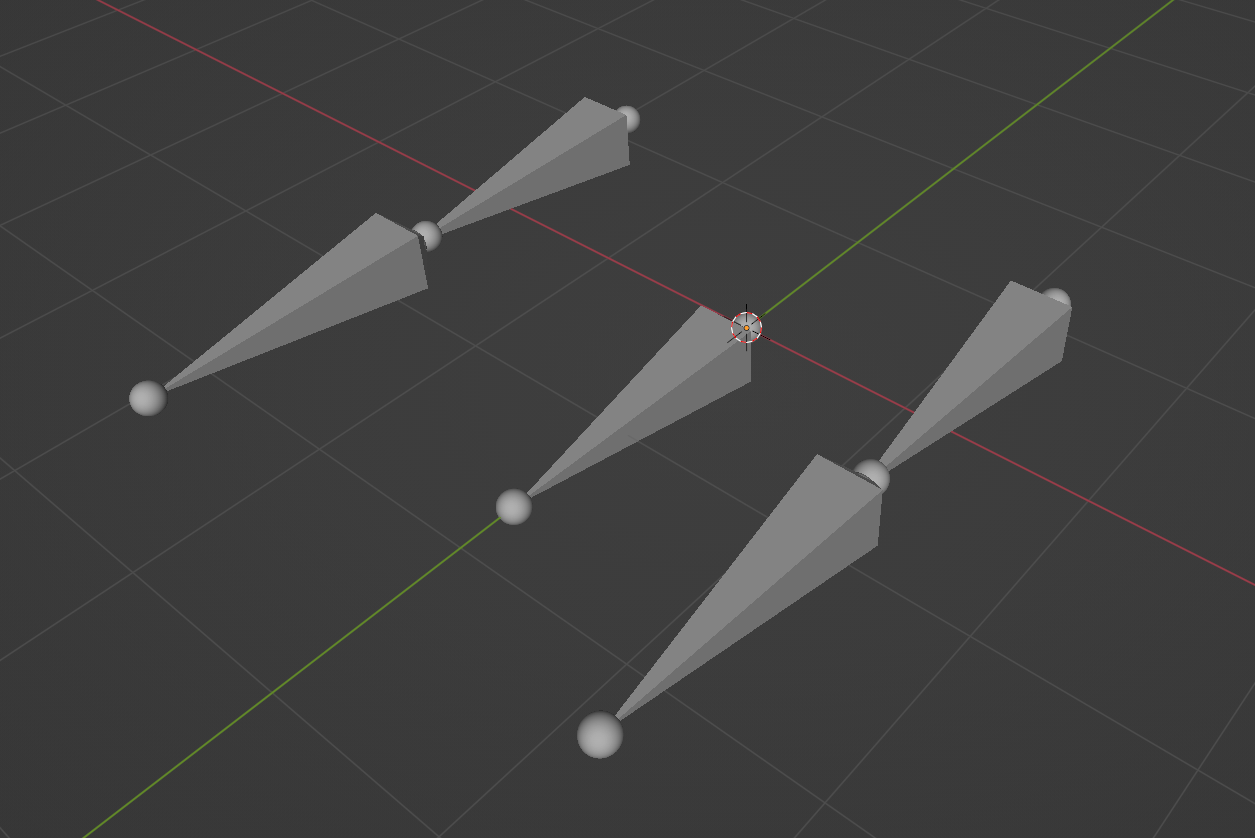
\includegraphics[width=0.4\textwidth]{resources/chapter-4/vehicle-skeleton.png}}
    \hfill
    \subfloat[Hierarki \textit{vehicle skeleton}]{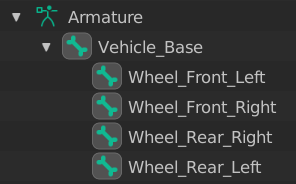
\includegraphics[width=0.4\textwidth]{resources/chapter-4/vehicle-skeleton-hierarchy.png}}
    \caption{\textit{Vehicle skeleton} kendaraan roda 4}
    \label{fig:vehicle-skeleton}
\end{figure}

\begin{figure}[!h]
    \centering
    \subfloat[Tampak depan roda depan kiri angkot]{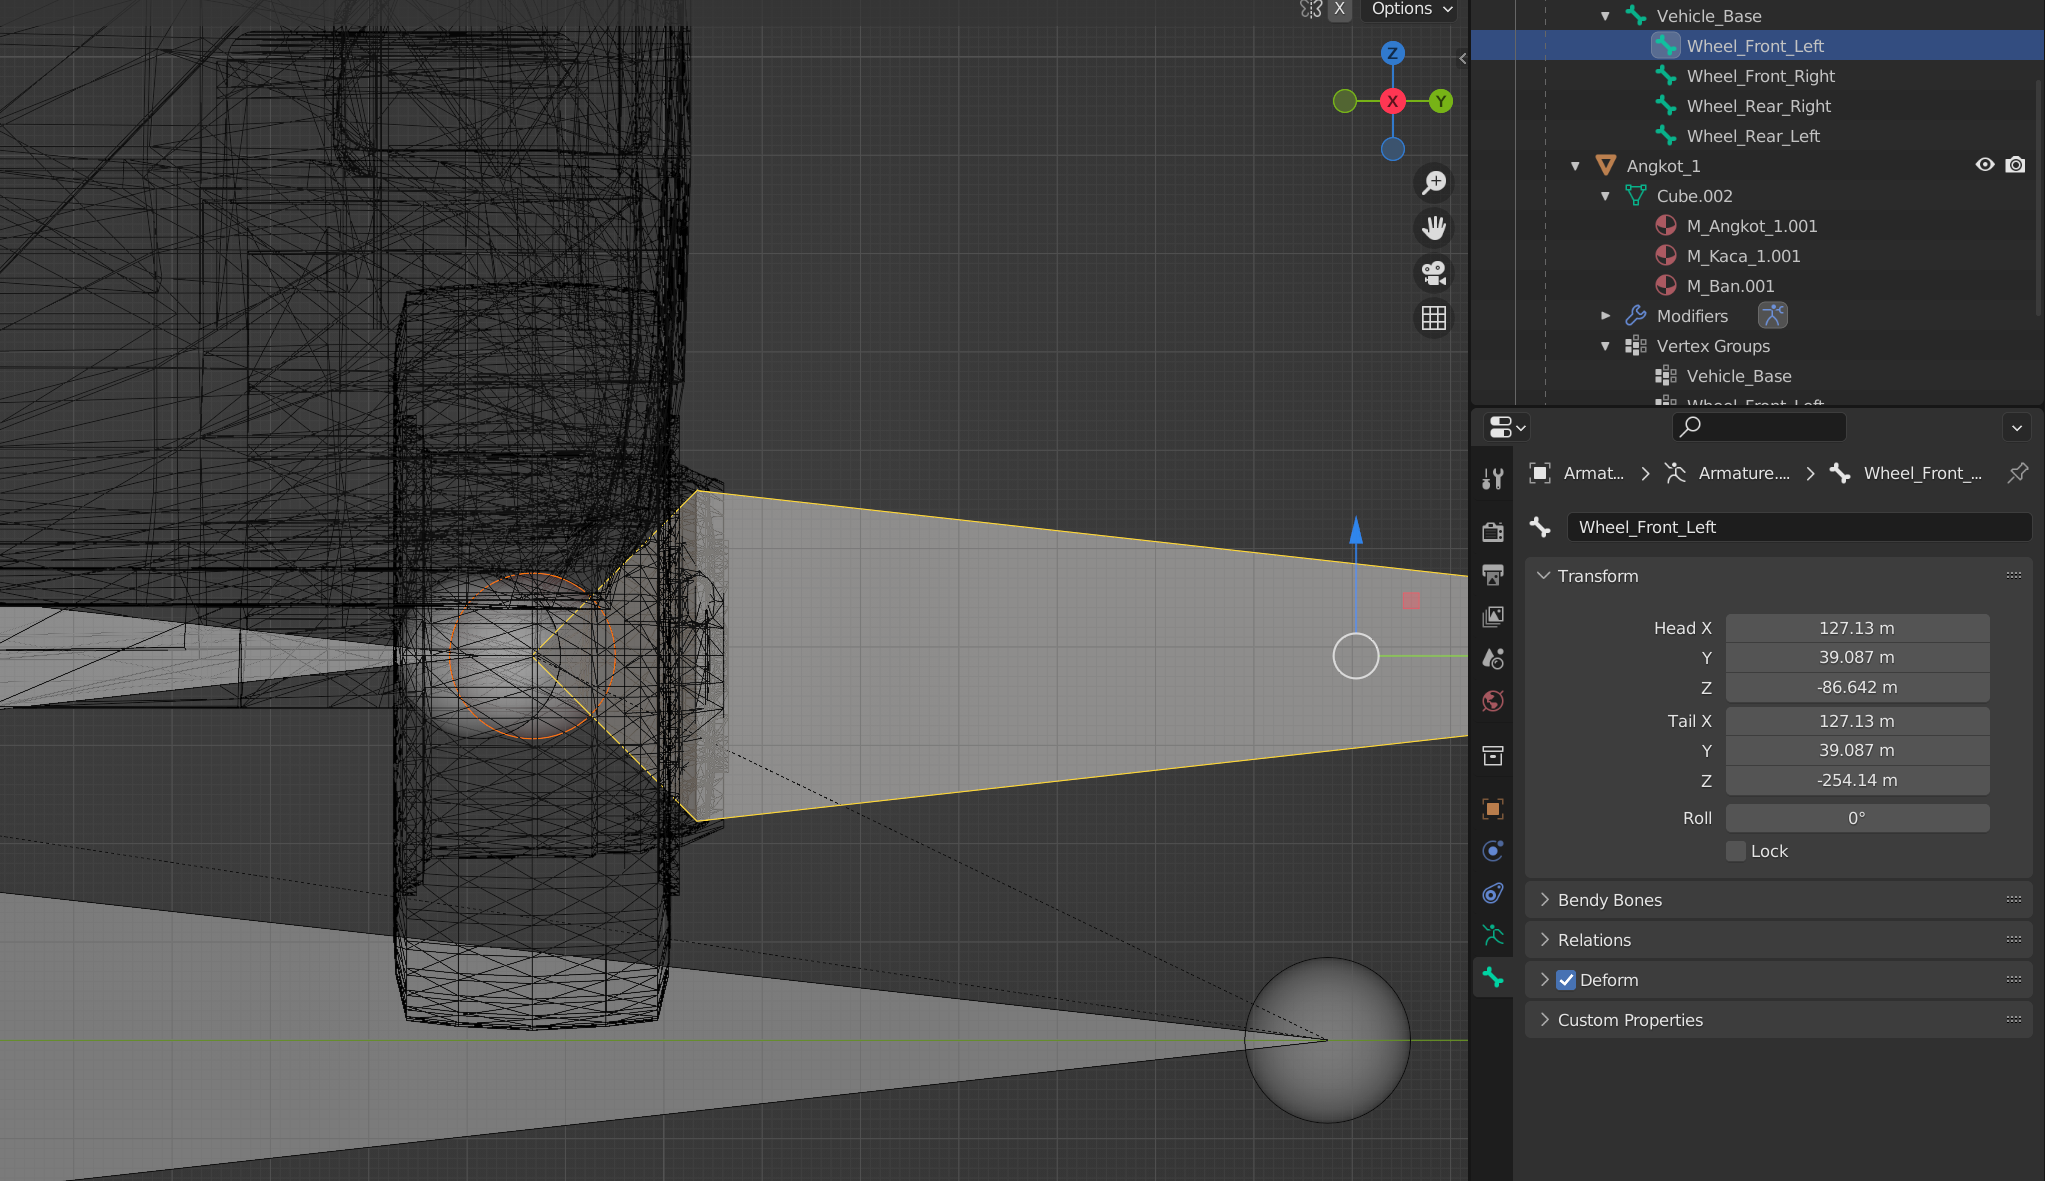
\includegraphics[width=0.45\textwidth]{resources/chapter-4/bone-placement-1.png}}
    \hfill
    \subfloat[Tampak samping roda depan kiri angkot]{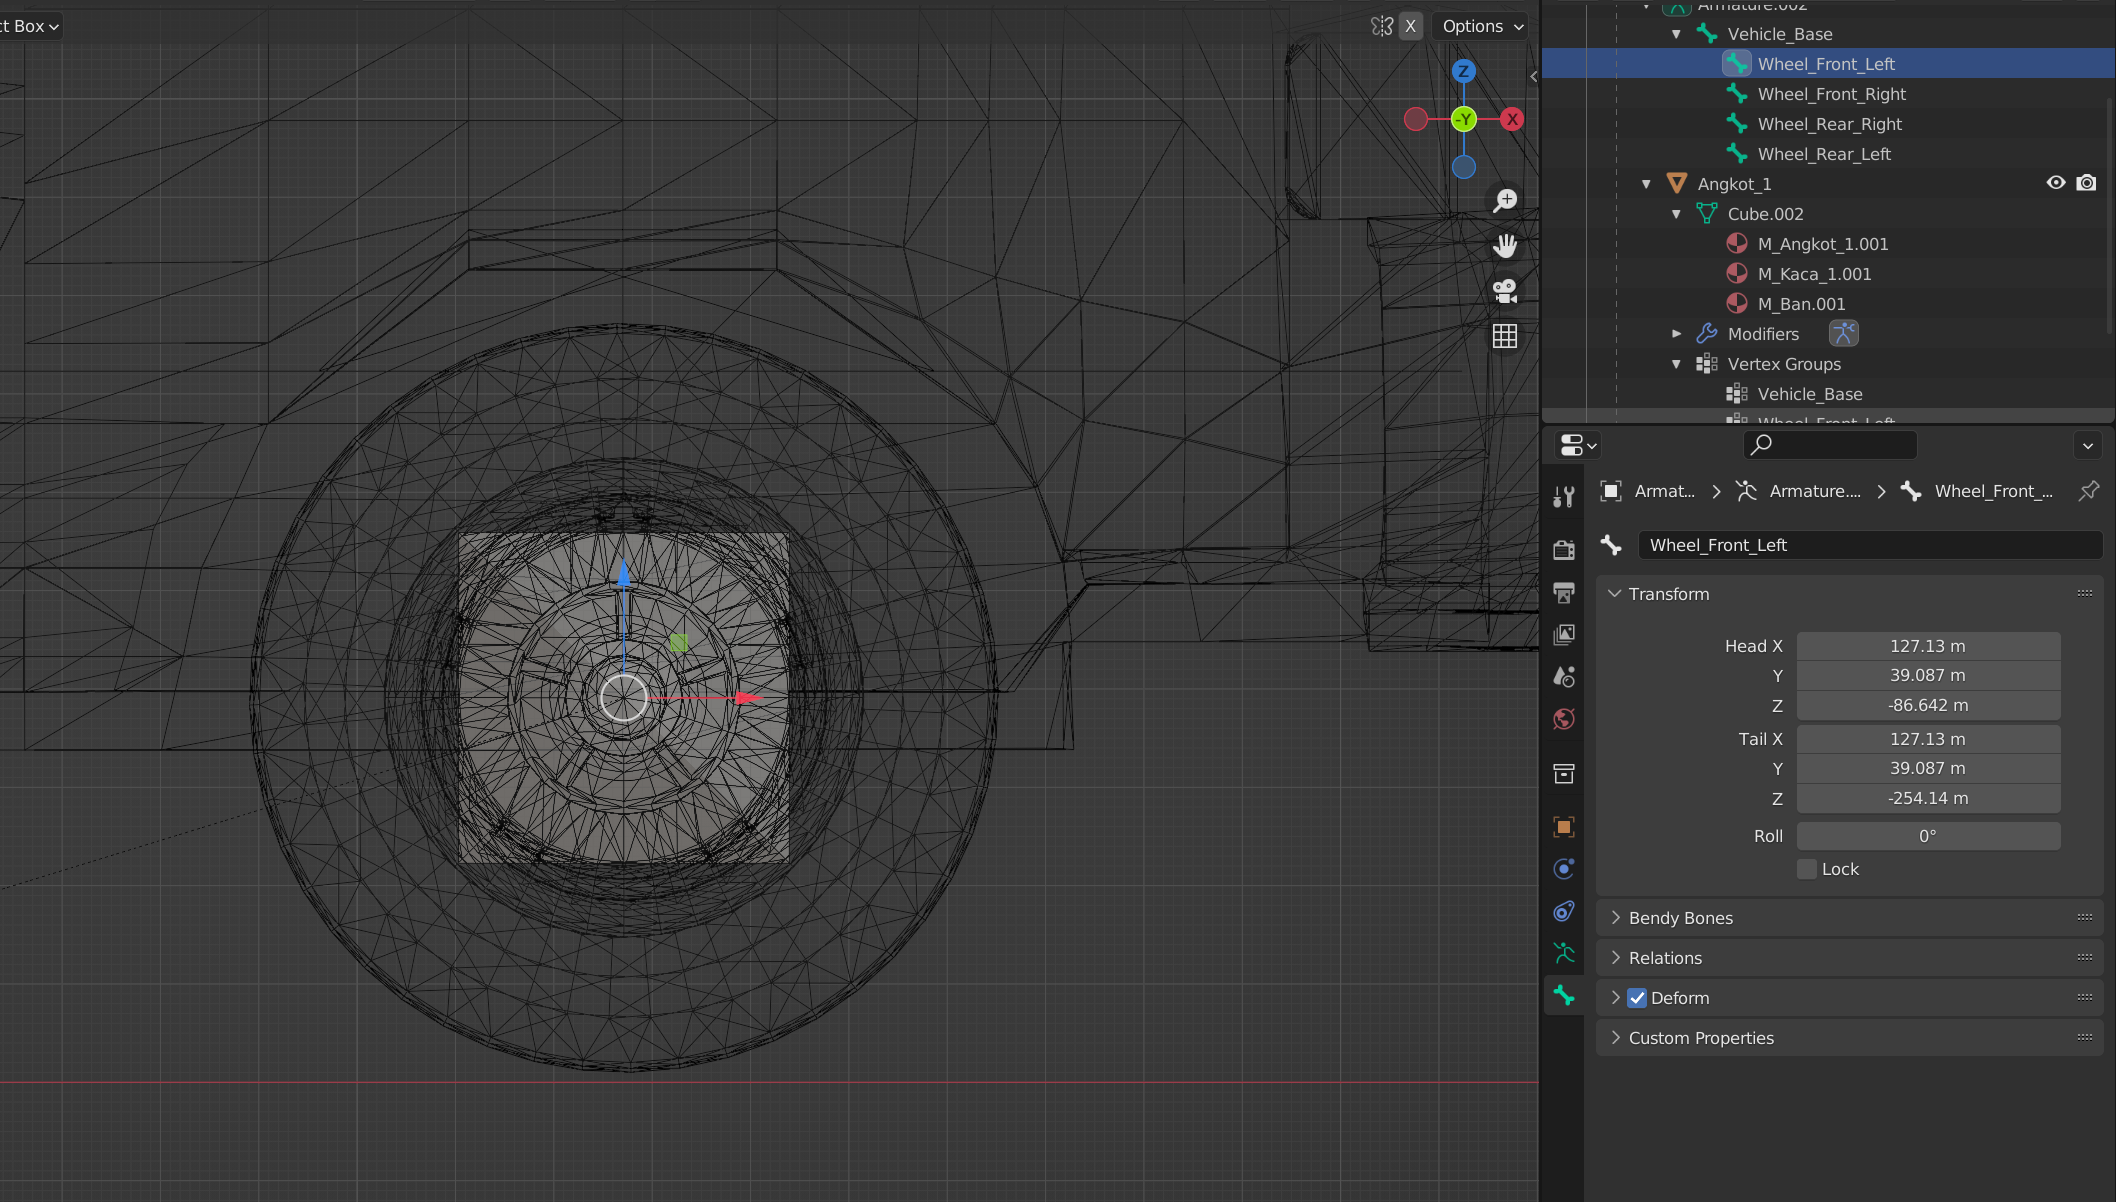
\includegraphics[width=0.45\textwidth]{resources/chapter-4/bone-placement-2.png}}
    \hfill
    \subfloat[Trem dengan \textit{armature} yang telah diatur posisinya]{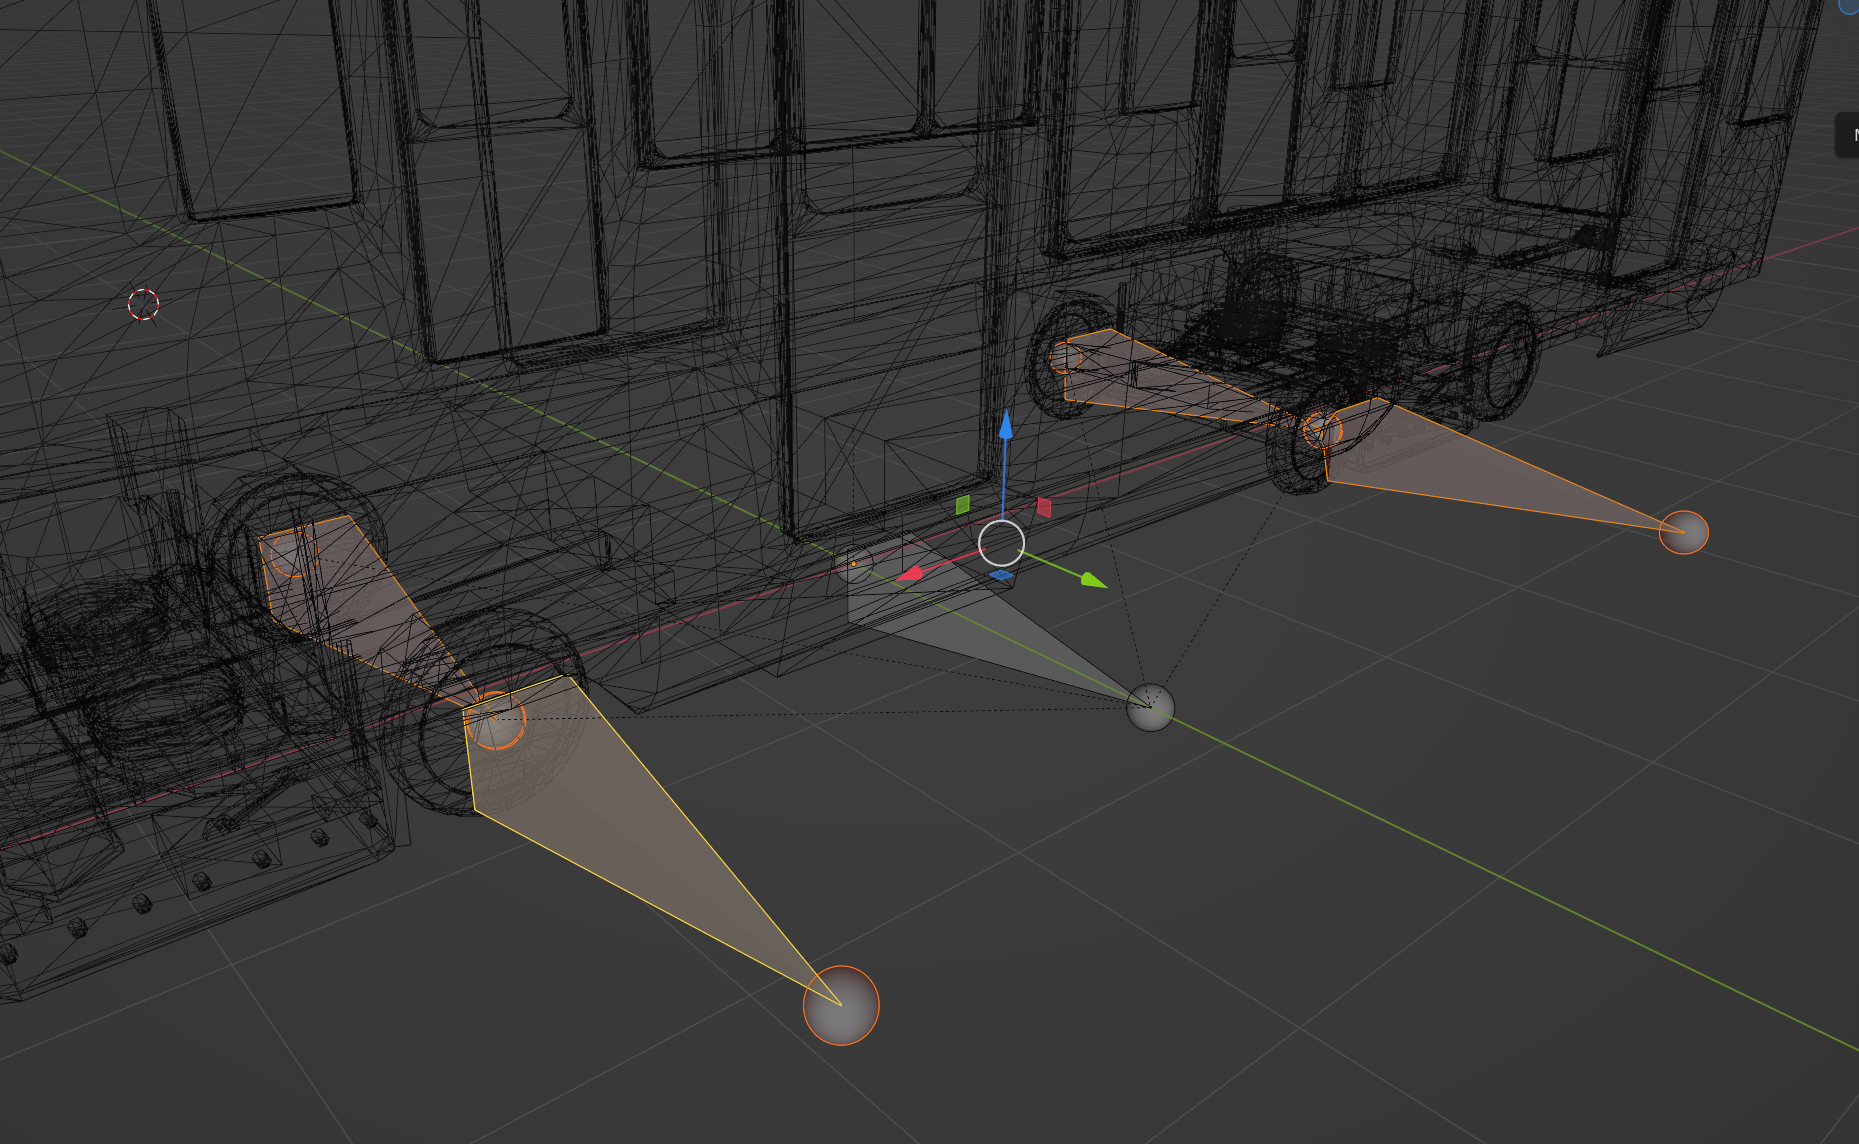
\includegraphics[width=0.45\textwidth]{resources/chapter-4/tram-wheels-bone.png}}
    \caption{Penempatan \textit{armature}}
    \label{fig:armature-placement}
\end{figure}

Setelah semua posisi \textit{bone} sesuai, dilakukan \textit{skinning} antara
\textit{armature} dengan \textit{mesh} kendaraan. Lima \textit{vertices groups}
dibuat untuk menghubungkan kumpulan titik dengan \textit{bone} yang sesuai.
Kelima \textit{vertices groups} dibuat dengan nama yang sesuai dengan nama
\textit{bone} yang akan dihubungkan. Gambar \ref{fig:vertices-groups}
menunjukkan \textit{vertices groups} yang sudah dibuat dan ditambahkan kumpulan
titiknya. \textit{Vertices groups} dibuat dengan cara memasuki \textit{edit
mode} (pada mesh kendaraan) dan menambahkan \textit{vertices groups} pada
\textit{tab} \verb|Object Data Properties|. Setelah itu, \textit{vertices
groups} tersebut diisi dengan titik-titik yang sesuai.

\begin{figure}[!h]
    \centering
    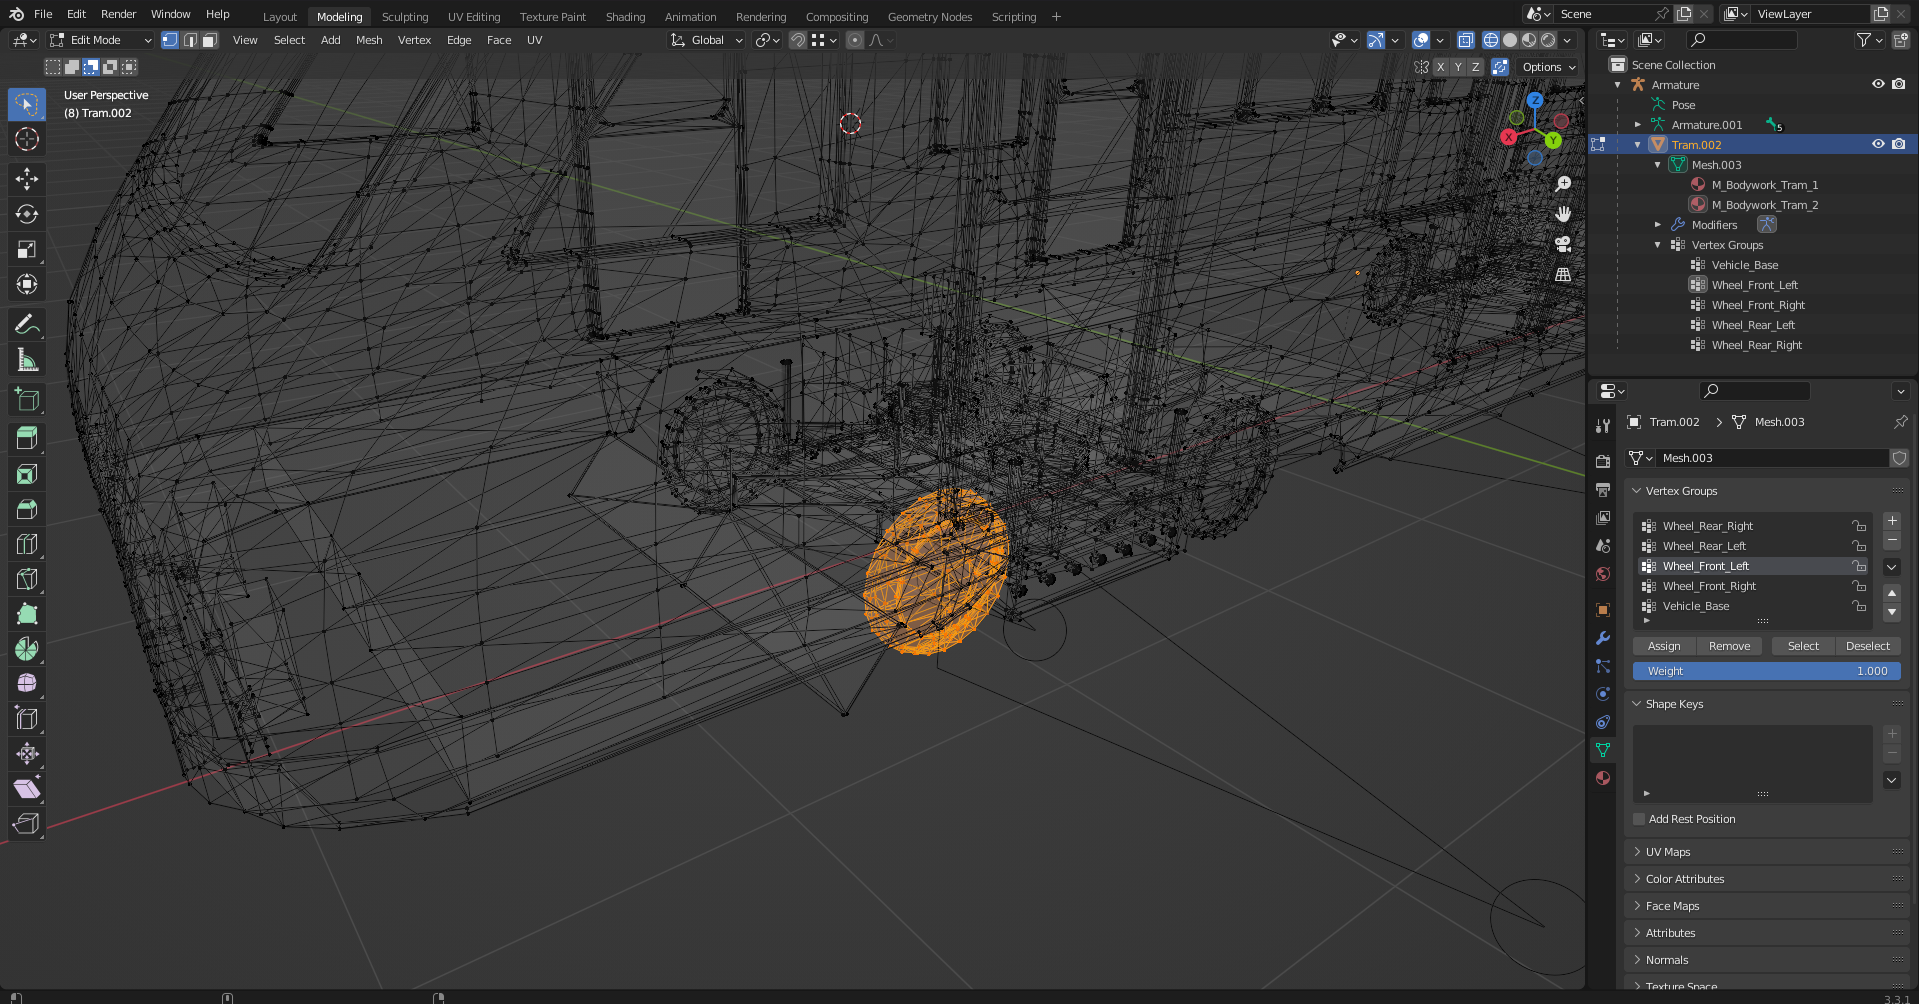
\includegraphics[width=1\textwidth]{resources/chapter-4/vertices-groups.png}
    \caption{\textit{Vertices groups} yang telah dibuat}
    \label{fig:vertices-groups}
\end{figure}

Dilakukan \textit{skinning} dengan cara memasuki \textit{object mode} dan
menyusun hierarki objek seperti pada Gambar \ref{fig:skinning-hierarchy}
kemudian memilih menu \verb|Object > Parent > Armature Deform with Automatic|
yang terletak pada \textit{Viewport Header}. Gambar \ref{fig:wheel-skinning}
menunjukkan roda angkot bagian depan kiri yang sudah dihubungkan dengan
\textit{bone} yang sesuai. Pengujian ini dilakukan dengan memilih salah satu
\textit{bone}, mengetik `r', dan menggerakan \textit{cursor} pada \textit{pose
mode}.

\begin{figure}[!h]
    \centering
    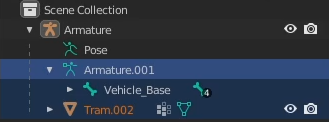
\includegraphics[width=0.6\textwidth]{resources/chapter-4/skinning-hierarchy.png}
    \caption{Hierarki objek}
    \label{fig:skinning-hierarchy}
\end{figure}

\begin{figure}[!h]
    \centering
    \subfloat[Roda posisi awal]{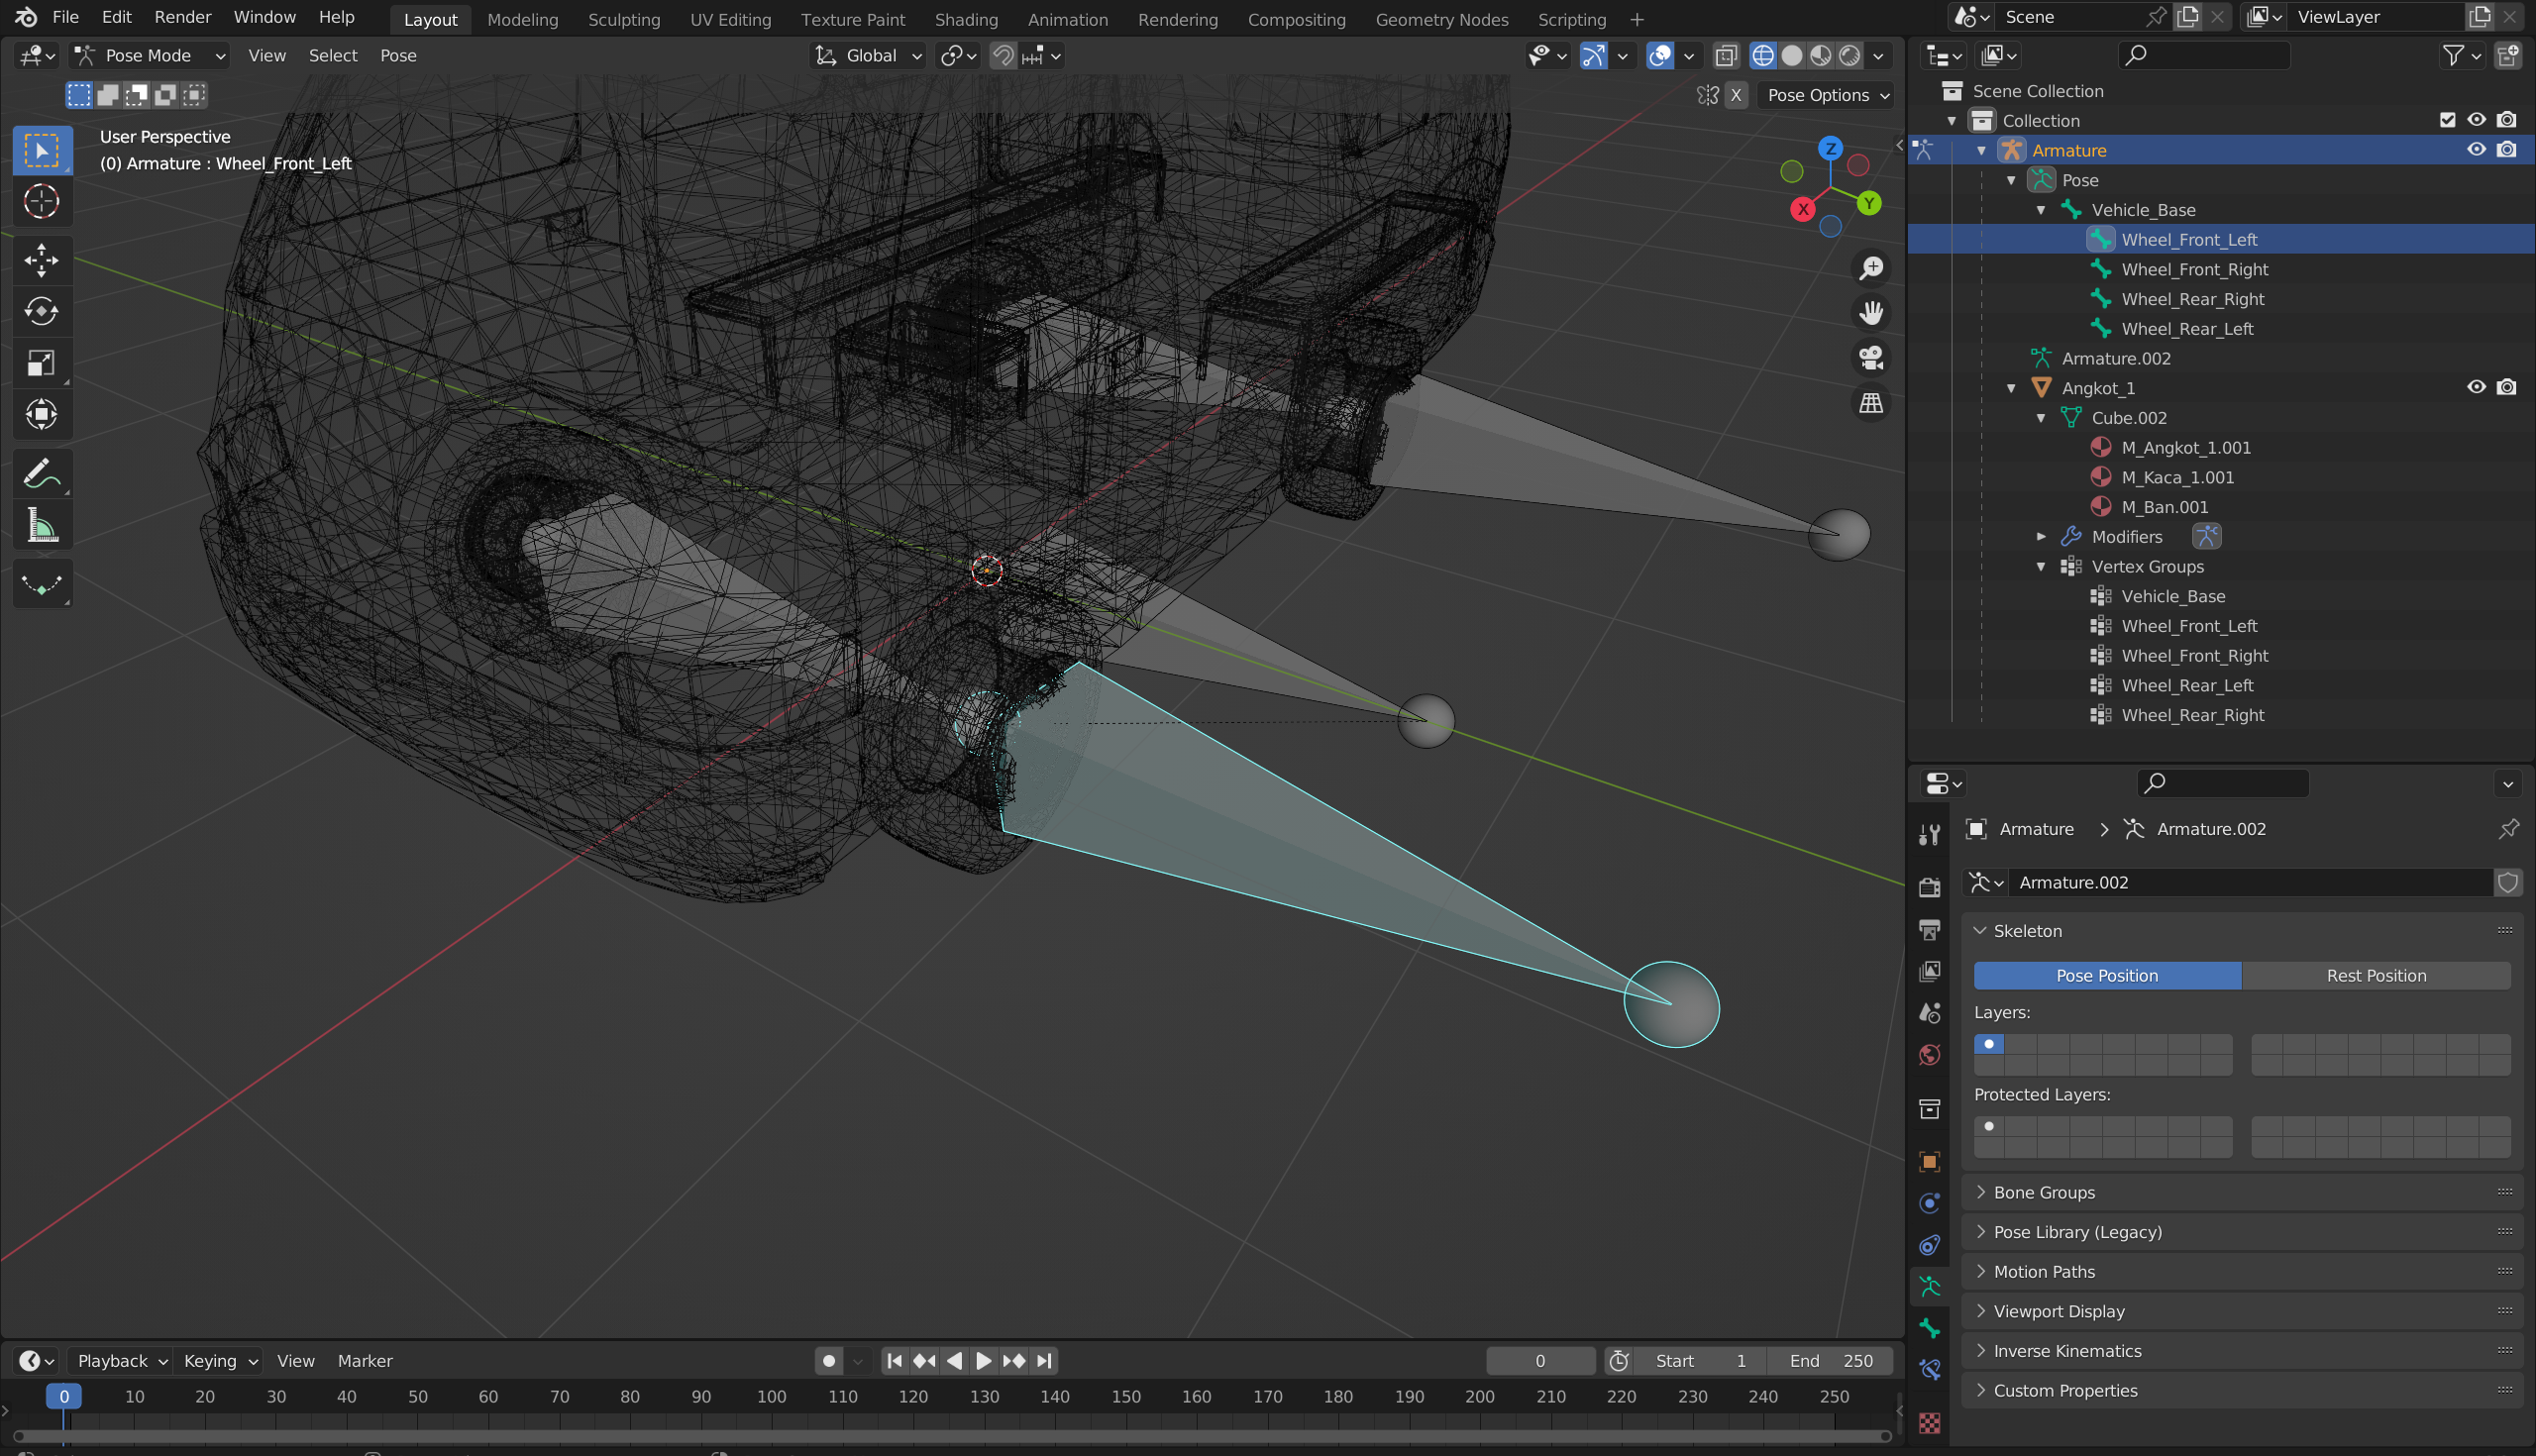
\includegraphics[width=0.47\textwidth]{resources/chapter-4/skinned-wheel-default.png}}
    \hfill
    \subfloat[Perubahan posisi roda]{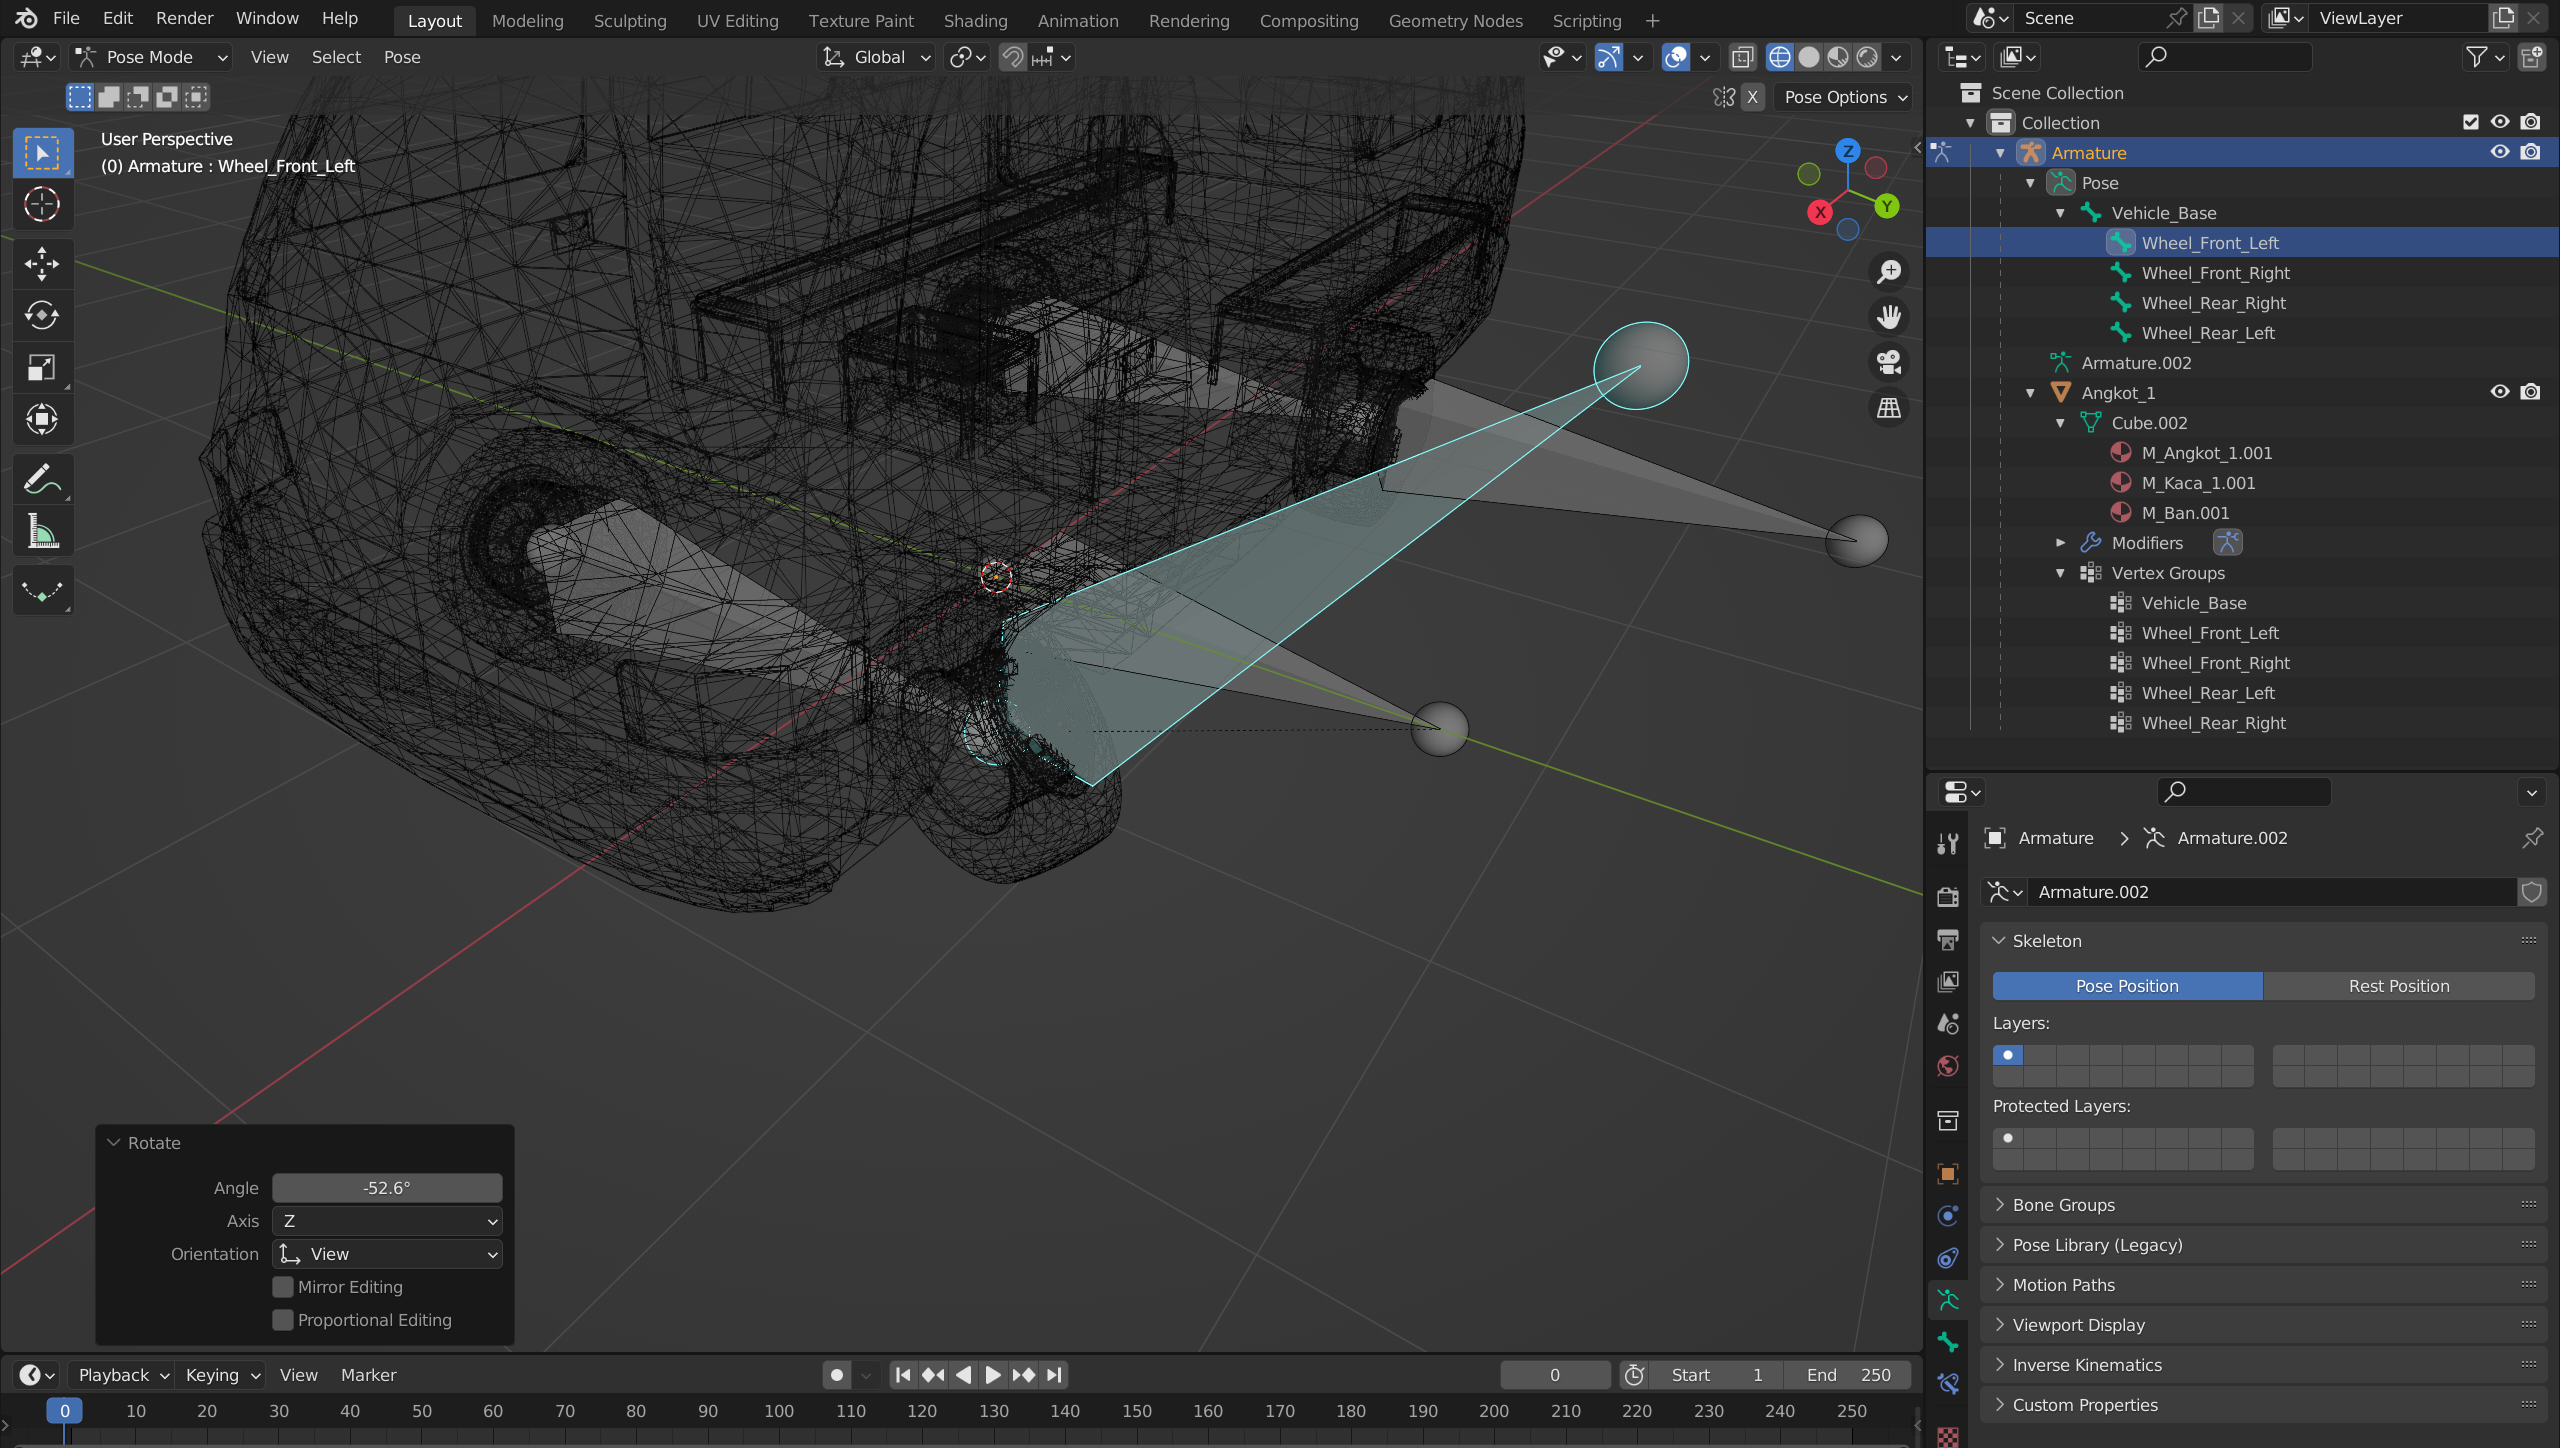
\includegraphics[width=0.47\textwidth]{resources/chapter-4/skinned-wheel-moved.png}}
    \caption{Hasil \textit{skinning} roda yang benar}
    \label{fig:wheel-skinning}
\end{figure}

Aset model 3D kemudian diekspor ke dalam format FBX. Gambar \ref{fig:export-fbx}
menunjukkan opsi ekspor yang digunakan. Opsi yang perlu diperhatikan adalah opsi
\verb|Forward| dan \verb|Up| pada bagian \verb|Transform|. Opsi \verb|Forward|
harus diatur ke arah sumbu \verb|-Z Forward| dan opsi \verb|Up| harus diatur ke
arah sumbu \verb|Y Up|. Opsi lainnya dapat diatur sesuai kebutuhan.

\begin{figure}[!h]
    \centering
    \subfloat[Opsi ekspor berkas FBX]{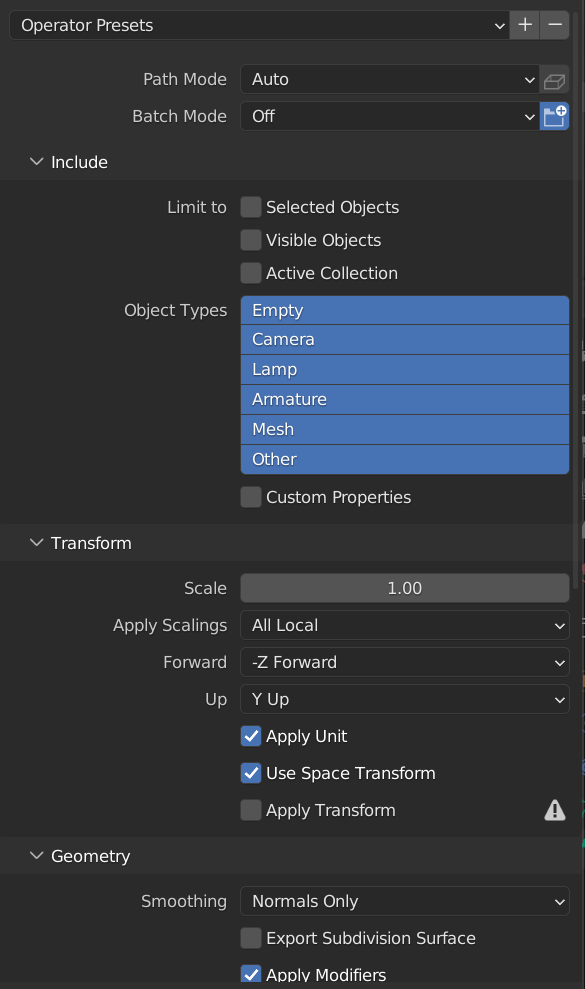
\includegraphics[width=0.47\textwidth]{resources/chapter-4/export-fbx-options-1.png}}
    \hfill
    \subfloat[Opsi ekspor berkas FBX lanjutan]{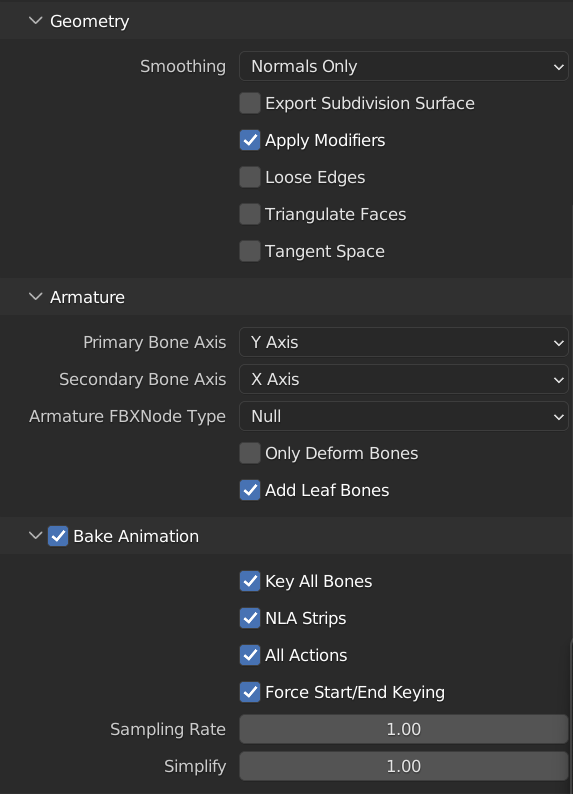
\includegraphics[width=0.47\textwidth]{resources/chapter-4/export-fbx-options-2.png}}
    \caption{Opsi ekspor berkas FBX}
    \label{fig:export-fbx}
\end{figure}

\subsubsection{Impor Berkas FBX Kendaraan Roda 4 ke dalam Editor CARLAUE4}

% TODO: add carlaue4 editor ui?

Setelah aset model 3D selesai dibuat dan diekspor ke dalam format FBX, berkas
FBX tersebut diimpor ke dalam editor CARLAUE4. Sebelum berkas FBX kendaraan
diimpor, sebuah \textit{folder} baru dibuat di dalam direktori
\verb|/Content/Carla/Static/Vehicles/4Wheeled| (selanjutnya akan disebut sebagai
\textit{folder} \verb|Static|) di \textit{Content Browser} kemudian berkas FBX
dapat diimpor ke dalam \textit{folder} tersebut dengan klik kanan pada
\textit{Content Browser}. Gambar \ref{fig:fbx-import-options-4wheeled}
menunjukkan opsi yang digunakan untuk mengimpor berkas FBX kendaraan roda 4.
Berikut adalah beberapa opsi yang perlu diperhatikan dan diatur:

\begin{enumerate}
    \item Opsi \verb|Import Content Type| harus diatur ke \texttt{Geometry and Skinning Weights}.
    \item Opsi \verb|Normal Import Method| harus diatur ke \verb|Import Normals|.
    \item Opsi \verb|Use T0 as Ref Pose| harus dicentang.
\end{enumerate}

\begin{figure}[!ht]
    \centering
    \subfloat[Opsi impor berkas FBX]{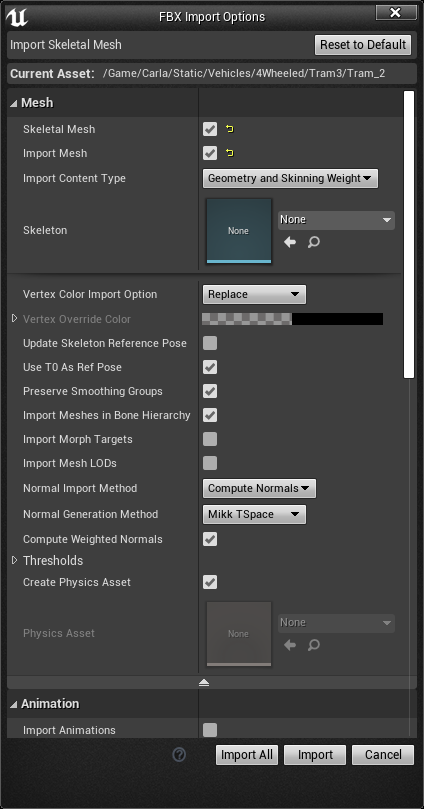
\includegraphics[width=0.47\textwidth]{resources/chapter-4/fbx-import-options-4wheeled-1.png}}
    \hfill
    \subfloat[Opsi impor berkas FBX lanjutan]{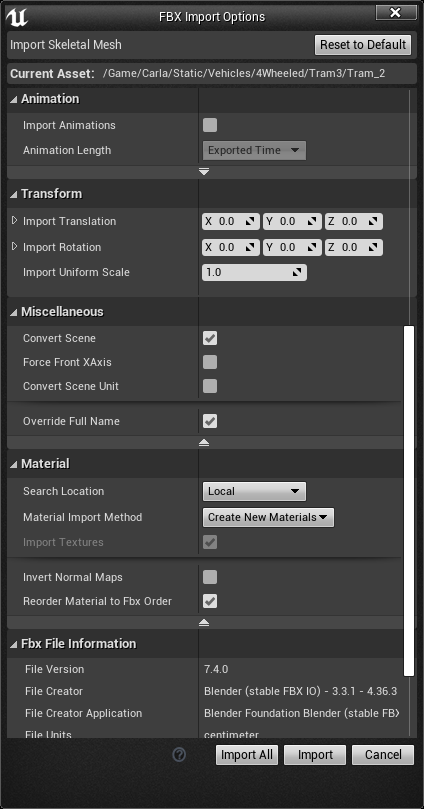
\includegraphics[width=0.47\textwidth]{resources/chapter-4/fbx-import-options-4wheeled-2.png}}
    \caption{Opsi impor berkas FBX kendaraan roda 4}
    \label{fig:fbx-import-options-4wheeled}
\end{figure}

Pengimporan berkas FBX tersebut menghasilkan aset-aset sebagai berikut:

\begin{enumerate}
    \item Aset \textit{skeletal mesh} \verb|<nama_kendaraan>|
    \item Aset \textit{skeleton} \verb|<nama_kendaraan>_Skeleton|
    \item Aset \textit{physics} \verb|<nama_kendaraan>_PhysicsAsset|
    \item Aset-aset material dan tekstur yang ada dalam berkas FBX jika opsi
    \verb|Material Import Method| diatur ke \verb|Create New Materials|.
\end{enumerate}

Aset \textit{physics} diedit agar sesuai dengan bentuk aset \textit{mesh}.
Bentuk \textit{body} badan kendaraan atau \textit{vehicle base} disesuaikan
dengan cara mengubah \verb|Primitive Type| menjadi \verb|Multi Convex Hull|
pada panel \verb|Tools|. Badan dari masing-masing roda kendaraan disesuaikan
bentuk \verb|Primitive Type|-nya menjadi \verb|Sphere|. Dilakukan pengaturan
opsi-opsi pada panel \verb|Details| untuk masing-masing roda, yaitu opsi
\verb|Linear Damping| diatur menjadi \verb|0| dan opsi \verb|Physics Type|
diatur menjadi \verb|Kinematic|. Opsi \verb|Simulation Generates Hit Events|
pada panel \verb|Details| dicentang untuk badan dan roda-roda kendaraan agar
\textit{collider} kendaraan dapat menghasilkan \textit{hit event}. Gambar
\ref{fig:physics-asset-4wheeled} menunjukkan aset \textit{physics} kendaraan
roda 4 sebelum dan setelah diedit.

\begin{figure}[!ht]
    \centering
    \subfloat[Aset \textit{physics} trem sebelum pengeditan]{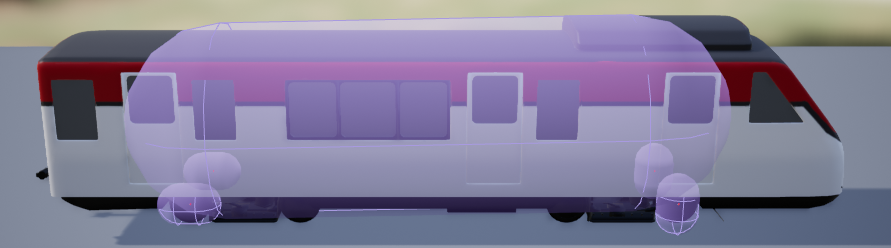
\includegraphics[width=0.6\textwidth]{resources/chapter-4/tram-physics-asset-before.png}}
    \hfill
    \subfloat[Aset \textit{physics} trem setelah pengeditan]{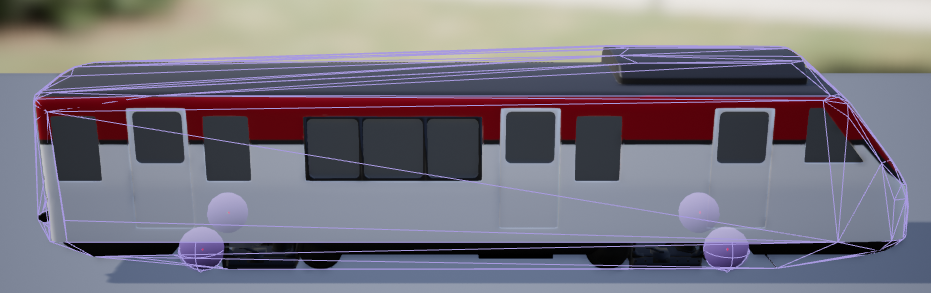
\includegraphics[width=0.6\textwidth]{resources/chapter-4/tram-physics-asset-after.png}}
    \caption{Aset \textit{physics} trem}
    \label{fig:physics-asset-4wheeled}
\end{figure}

Selain pengeditan aset \textit{physics}, dilakukan pembuatan aset \textit{static
mesh} dan berbagai aset \textit{blueprint} agar aset kendaraan dapat
mengintegrasikan sebagai kendaraan. Aset \textit{static mesh} dibuat dengan cara
menekan tombol \verb|Make Static Mesh| pada panel \verb|Toolbar| pada aset
\textit{skeletal mesh}. Aset tersebut dibuat untuk melengkapi \textit{static
mesh} yang tidak dibuat dalam Blender. Aset tersimpan pada direktori
\verb|/Content/Meshes/<nama_kendaraan>|.

Aset \textit{animation blueprint} dibuat untuk mengatur animasi kendaraan.
Karena semua animasi kendaraan roda 4 sama, aset \textit{animation blueprint}
dapat dibuat dengan menyalin isi aset \textit{animation blueprint} dari salah
satu kendaraan roda 4 yang sudah ada kemudian di-\textit{compile} dan disimpan
dengan nama \verb|AnimBP_<nama_kendaraan>|. Gambar
\ref{fig:blueprint-animation-4wheeled} menunjukkan aset \textit{animation
blueprint} trem.

\begin{figure}[!h]
    \centering
    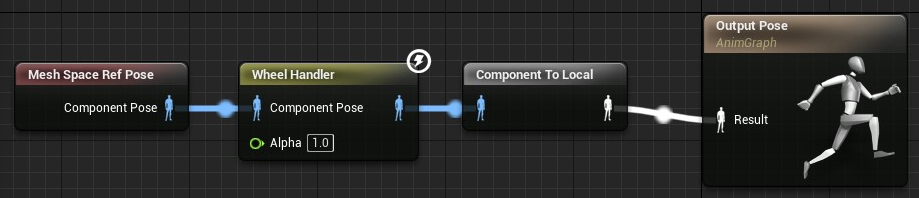
\includegraphics[width=1\textwidth]{resources/chapter-4/tram-animation-blueprint.png}
    \caption{Aset \textit{animation blueprint} trem}
    \label{fig:blueprint-animation-4wheeled}
\end{figure}

% note: blueprint animation can be explained more in detail

Aset-aset di dalam \textit{folder} \verb|Static| selesai dibuat. Gambar
\ref{fig:tram-assets-in-static-folder} menunjukkan aset-aset trem dalam
\textit{folder} \verb|Static|.

\begin{figure}[!h]
    \centering
    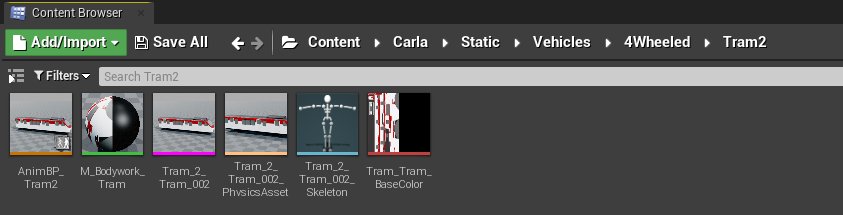
\includegraphics[width=1\textwidth]{resources/chapter-4/tram-assets-in-static-folder.png}
    \caption{Aset-aset trem dalam \textit{folder} \texttt{Static}}
    \label{fig:tram-assets-in-static-folder}
\end{figure}

Selanjutnya, dilakukan pembuatan aset dalam direktor
\verb|/Content/Carla/Bleprints/Vehicle/<nama_kendaraan>|.

% buat animation blueprint

% navigate ke bp folder
% buat folder baru
% buat bp roda, bp kendaraan + configs

% add dto vehicle factory

% spawn vehicle (implemented but does it work?)

% TODO: trouble shooting? hal2 yang harus diperhatikan

Gambar \ref{fig:tram-carla} menunjukkan hasil implementasi trem. Gambar
\ref{fig:angkot-carla} menunjukkan hasil implementasi trem  angkot.

\begin{figure}[!h]
    \centering
    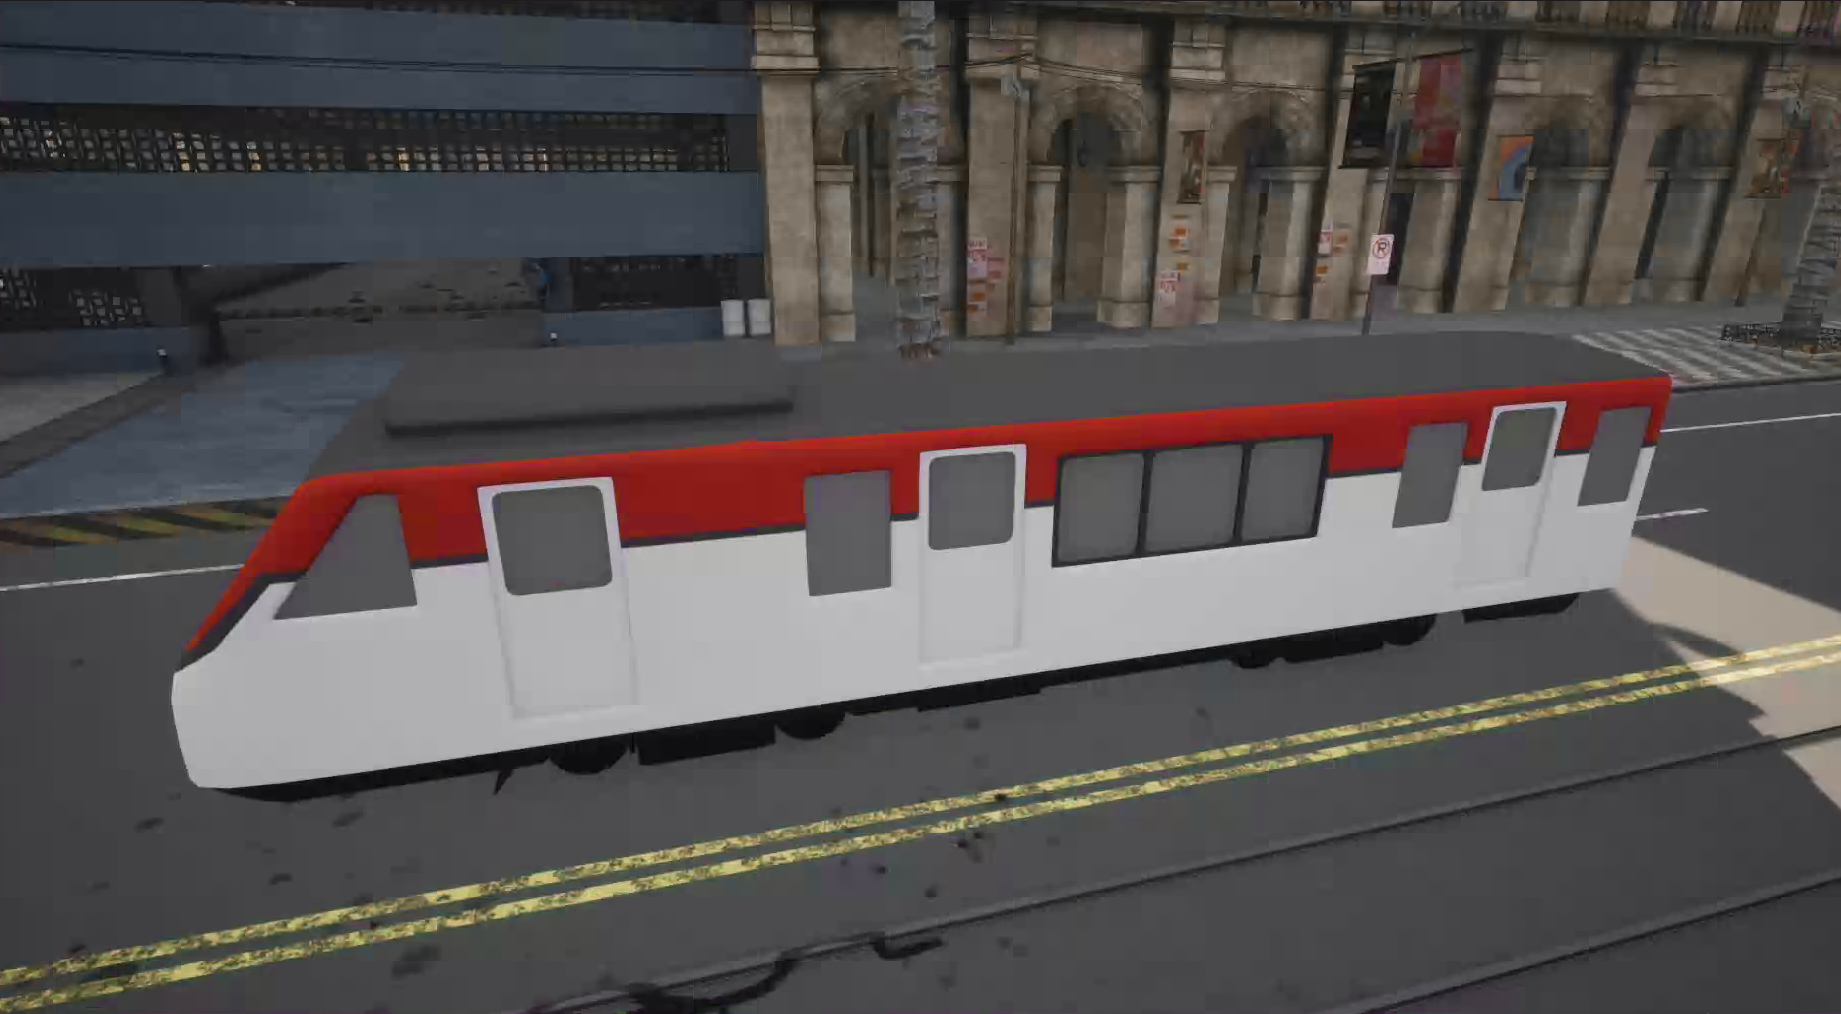
\includegraphics[width=0.6\textwidth]{resources/chapter-4/tram-carla.png}
    \caption{Implementasi trem dalam lingkungan simulasi}
    \label{fig:tram-carla}
\end{figure}

\begin{figure}[!h]
    \centering
    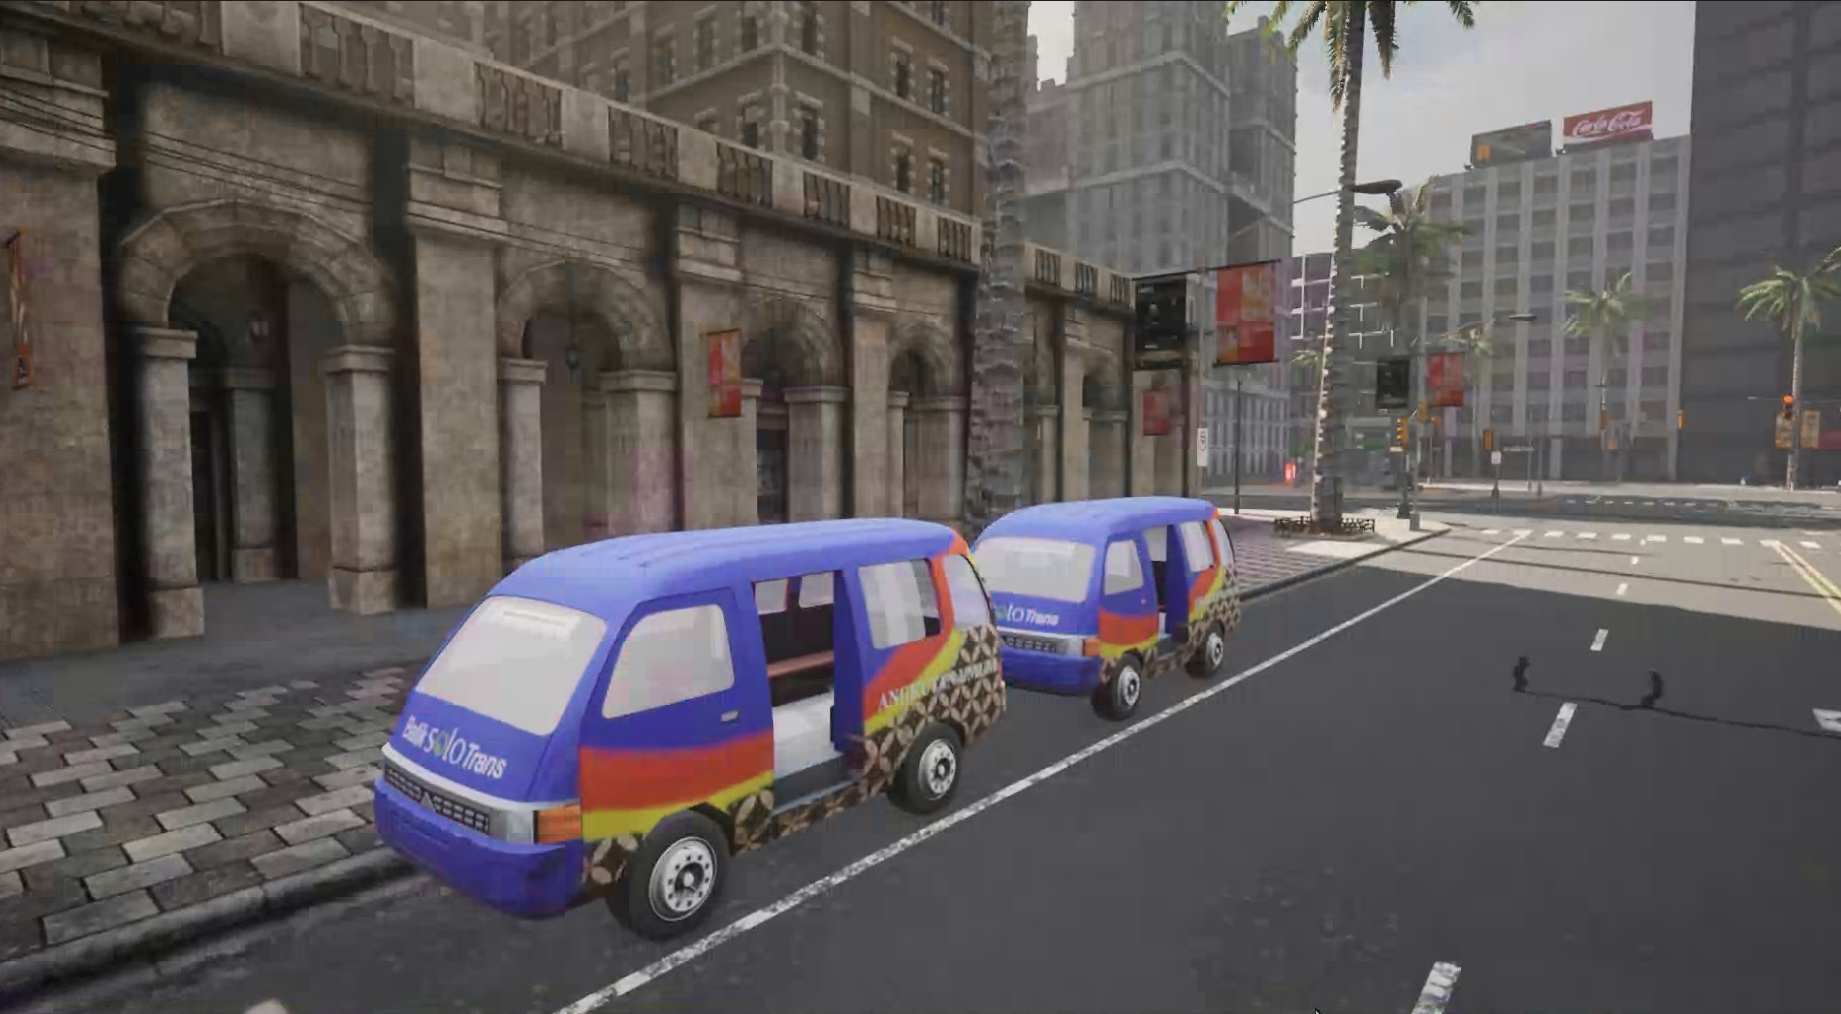
\includegraphics[width=0.6\textwidth]{resources/chapter-4/angkot.png}
    \caption{Implementasi angkot dalam lingkungan simulasi}
    \label{fig:angkot-carla}
\end{figure}

\subsection{Implementasi Sepeda Onthel, Sepeda Motor, dan Becak}

% TODO:
% \subsubsection{Pembuatan Aset Model 3D untuk Ekspor berkas FBX}
% \subsubsection{Impor Berkas FBX ke Editor CARLAUE4}

\subsection{Implementasi Lingkungan}

% TODO: ? cara import aset yang lain (yang khusus, yang detail di bawah aja)
% TODO: should i change the paragraph below into a subsubsection?

Penambahan aset model 3D ke dalam lingkungan simulasi dilakukan dengan membuat
folder baru pada direktori yang bersangkutan kemudian mengimpor aset model 3D ke
dalam folder tersebut. Cara menambahkan objek-objek statis ini adalah dengan
menarik objek dari impor dari \textit{Content Browser} ke dalam \textit{World
Outliner}. Setelah itu, dapat dilakukan penyesuaian skala, posisi, dan rotasi
aset pada \textit{World Outliner}. Penyesuaian lingkungan dapat dilakukan dengan
memilih dan mengaktifkan tingkat atau level objek yang ingin diubah.

% TODO: insert images, add directories, world levels, world outliner kah istilahnya?
% penyesuiannya lingkungan?

% TODO: benerin kata2nya jelek banget astaga

\subsubsection{Stasiun Madiun dan Stasiun Solokota}
% TODO: remove lihat gambar, figures need to be mentioned explicitly
Gambar \ref{fig:stasiun-madiun} menunjukkan implementasi model Stasiun Madiun
(lihat Gambar \ref{fig:stasiun-madiun-model}). Model stasiun kemudian
disesuaikan ukurannya dan diposisikan pada ... .

Gambar \ref{fig:stasiun-solokota} menunjukkan implementasi model Stasiun Solokota
(lihat Gambar \ref{fig:stasiun-solokota-model}). Model stasiun kemudian
disesuaikan ukurannya dan diposisikan pada ... .

% TODO: ..., + cara,  ke bab 3?

\begin{figure}[!h]
    \centering
    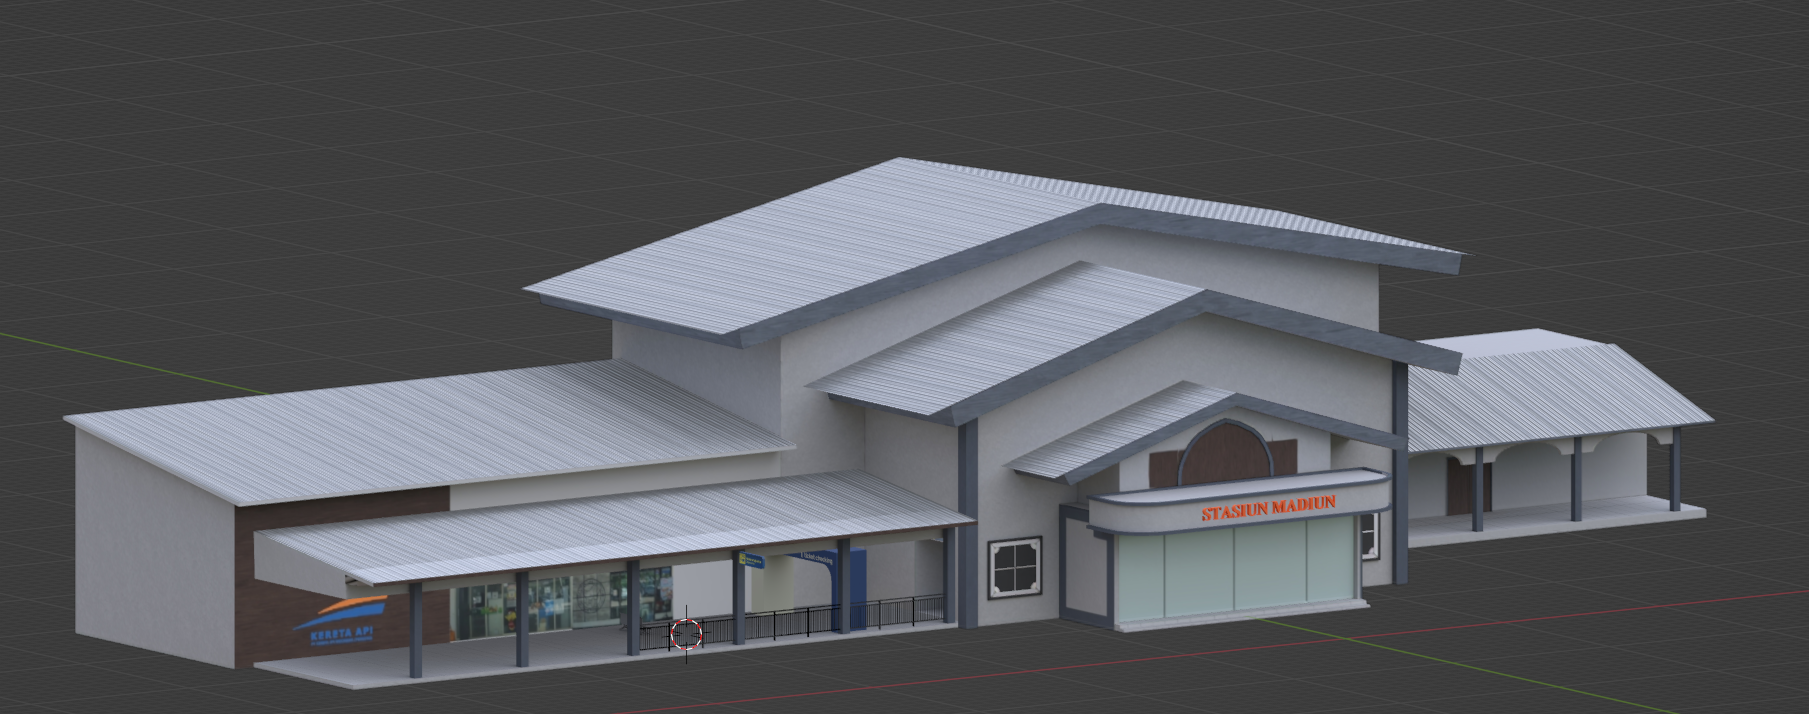
\includegraphics[width=0.6\textwidth]{resources/chapter-3-stasiun-madiun-model.png}
    \caption{Model Stasiun Madiun}
    \label{fig:stasiun-madiun-model}
\end{figure}

\begin{figure}[!h]
    \centering
    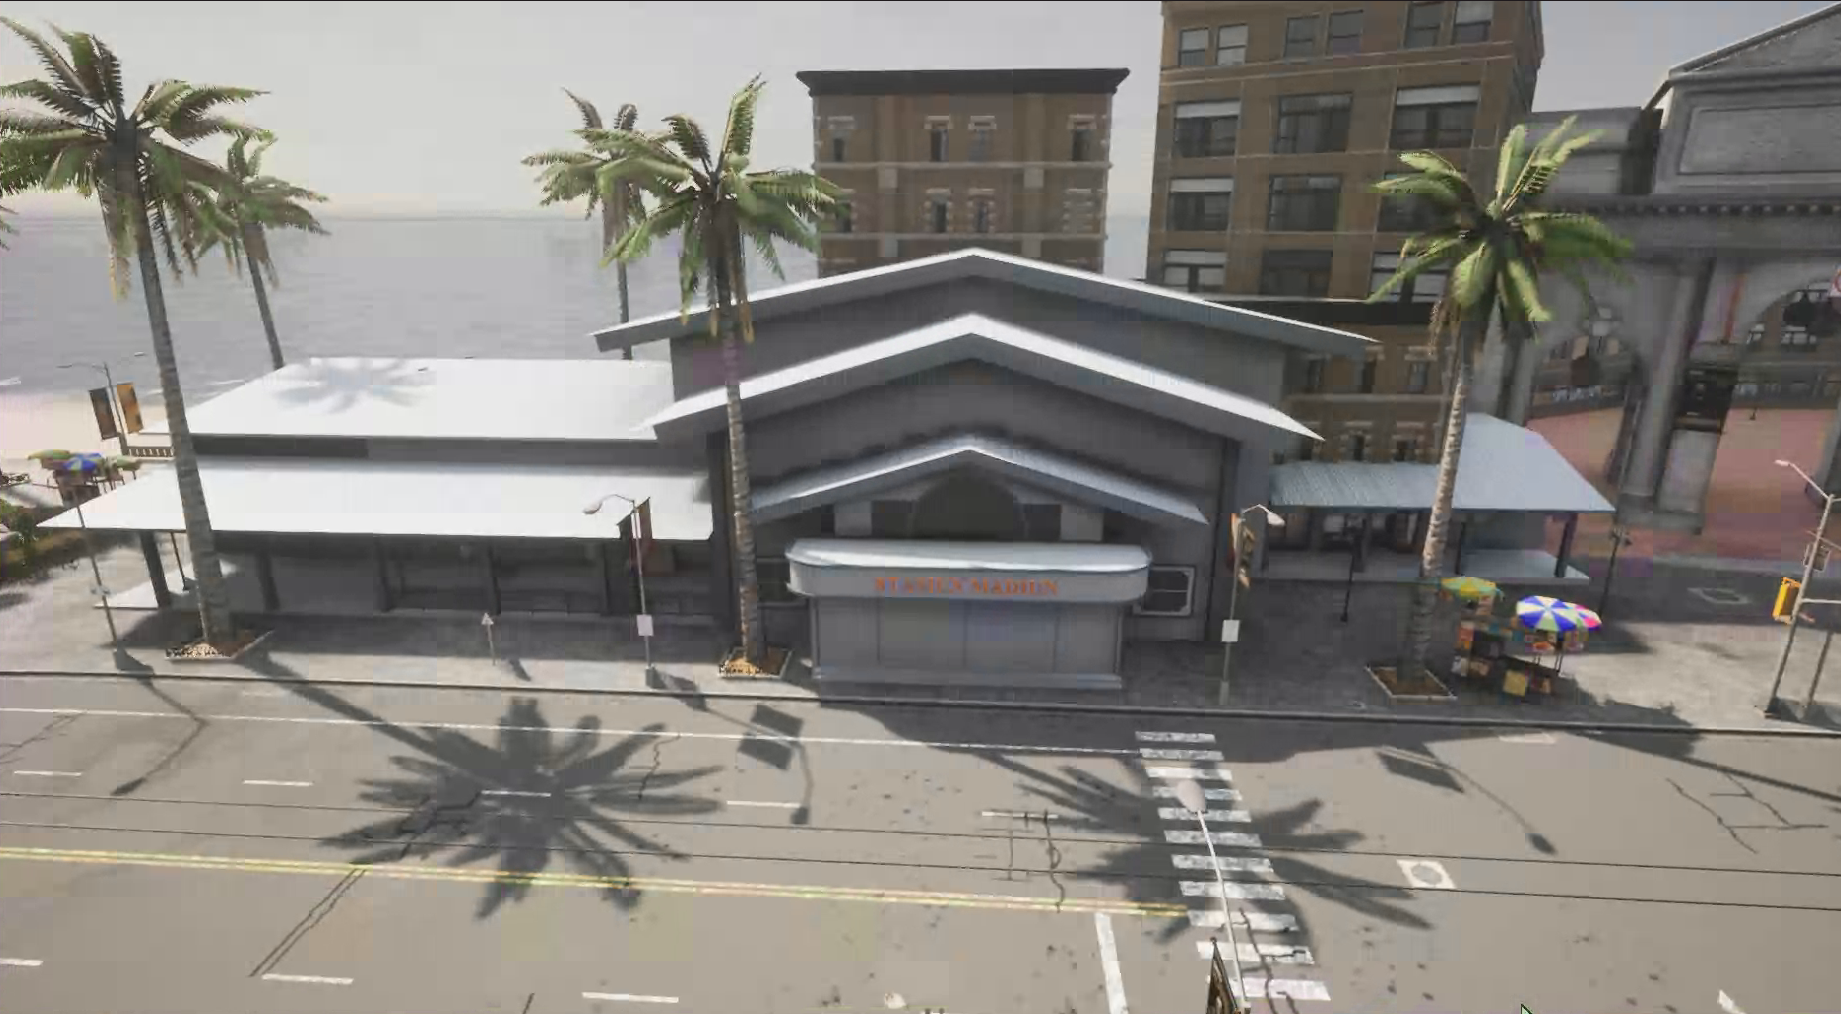
\includegraphics[width=0.6\textwidth]{resources/chapter-4/stasiun-madiun-carla.png}
    \caption{Implementasi stasiun Madiun dalam lingkungan simulasi}
    \label{fig:stasiun-madiun}
\end{figure}

\begin{figure}[!h]
    \centering
    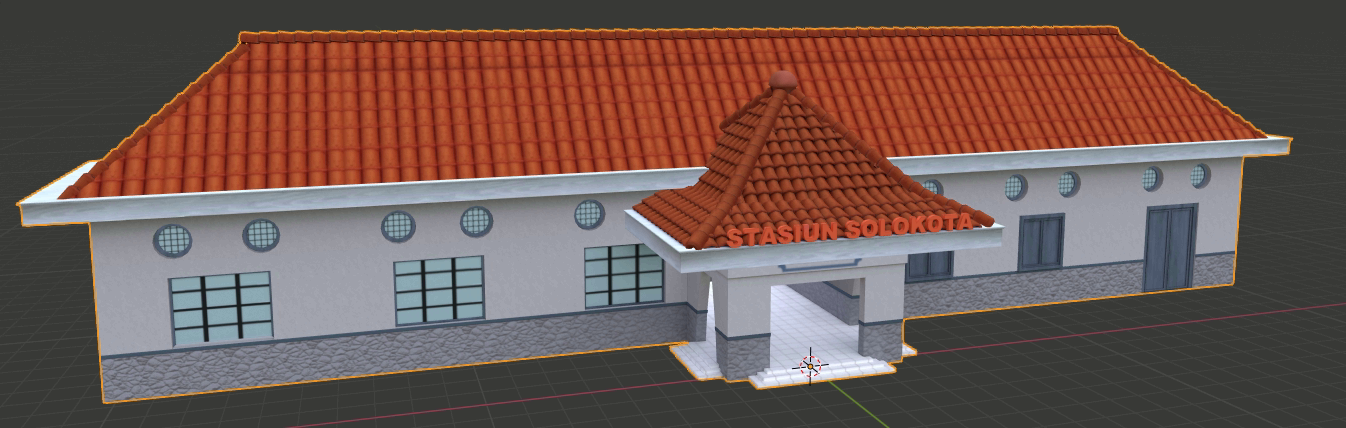
\includegraphics[width=0.6\textwidth]{resources/chapter-3-stasiun-solokota-model.png}
    \caption{Model Stasiun Solokota}
    \label{fig:stasiun-solokota-model}
\end{figure}

\begin{figure}[!h]
    \centering
    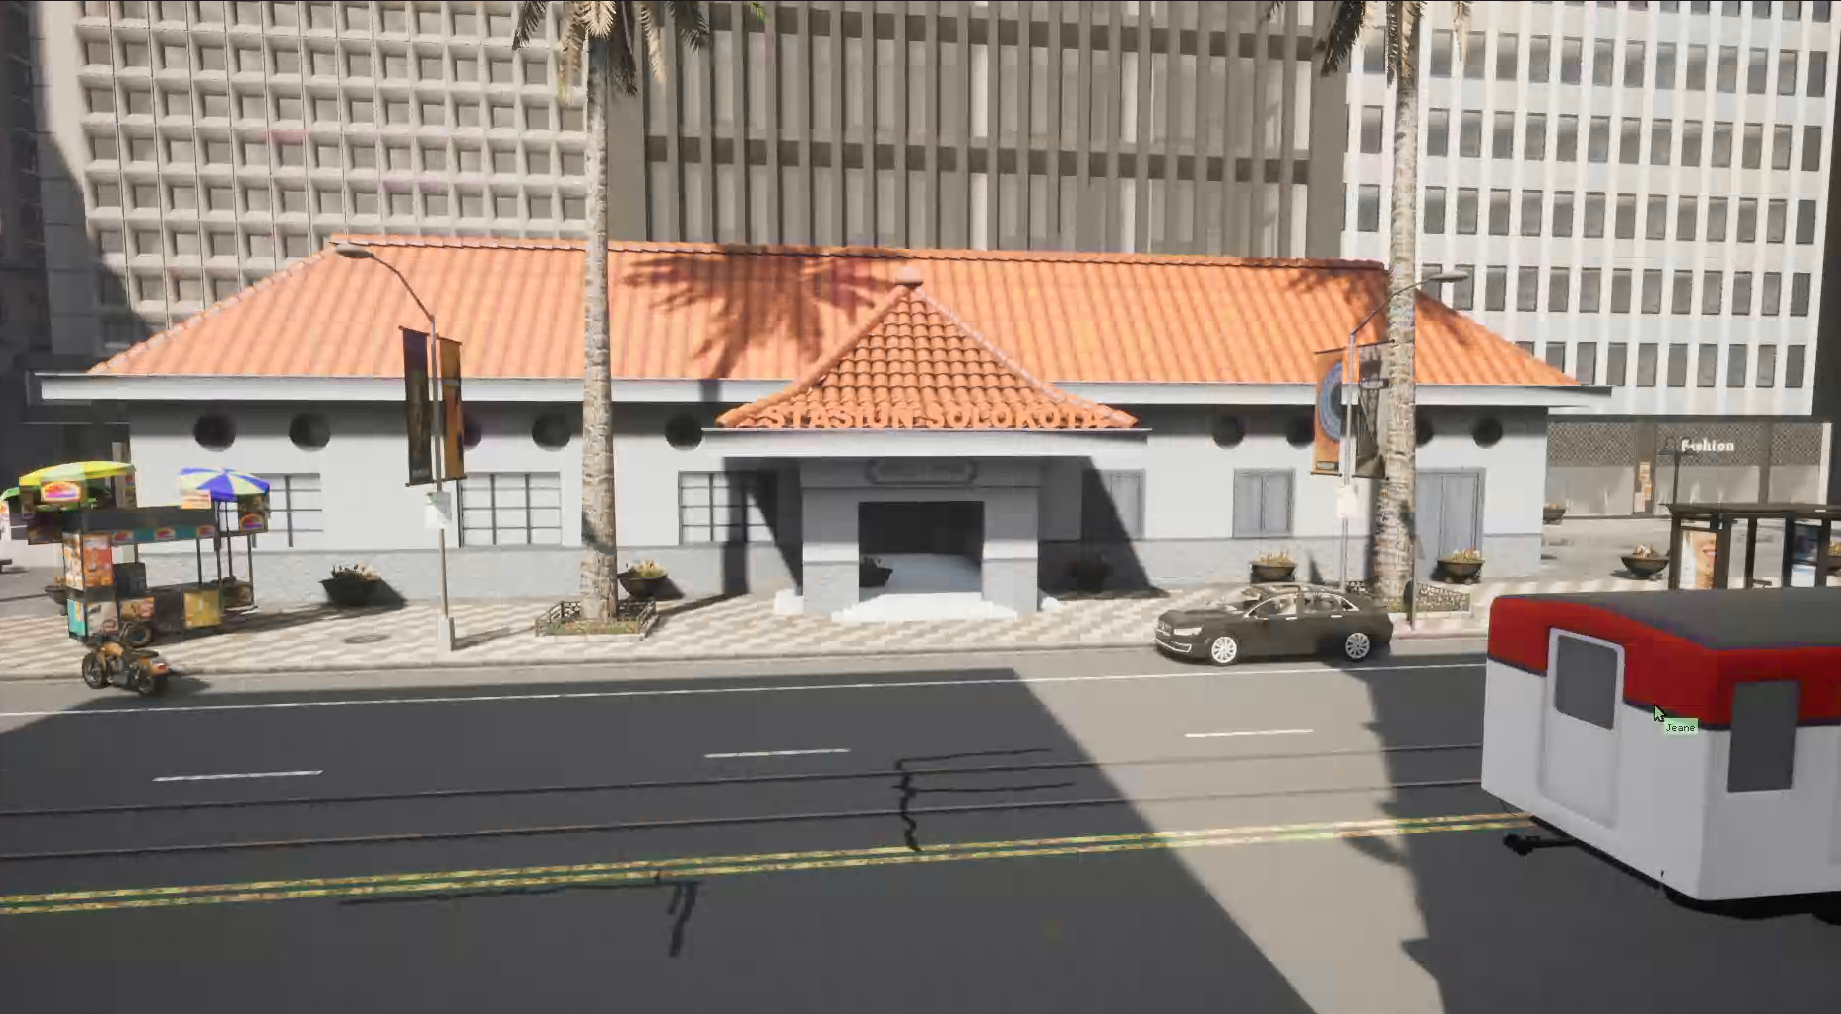
\includegraphics[width=0.6\textwidth]{resources/chapter-4/stasiun-solokota-carla.png}
    \caption{Implementasi stasiun Solokota dalam lingkungan simulasi}
    \label{fig:stasiun-solokota}
\end{figure}

\subsubsection{Rambu-rambu Lalu Lintas}

\begin{figure}[!h]
    \centering
    \subfloat[]{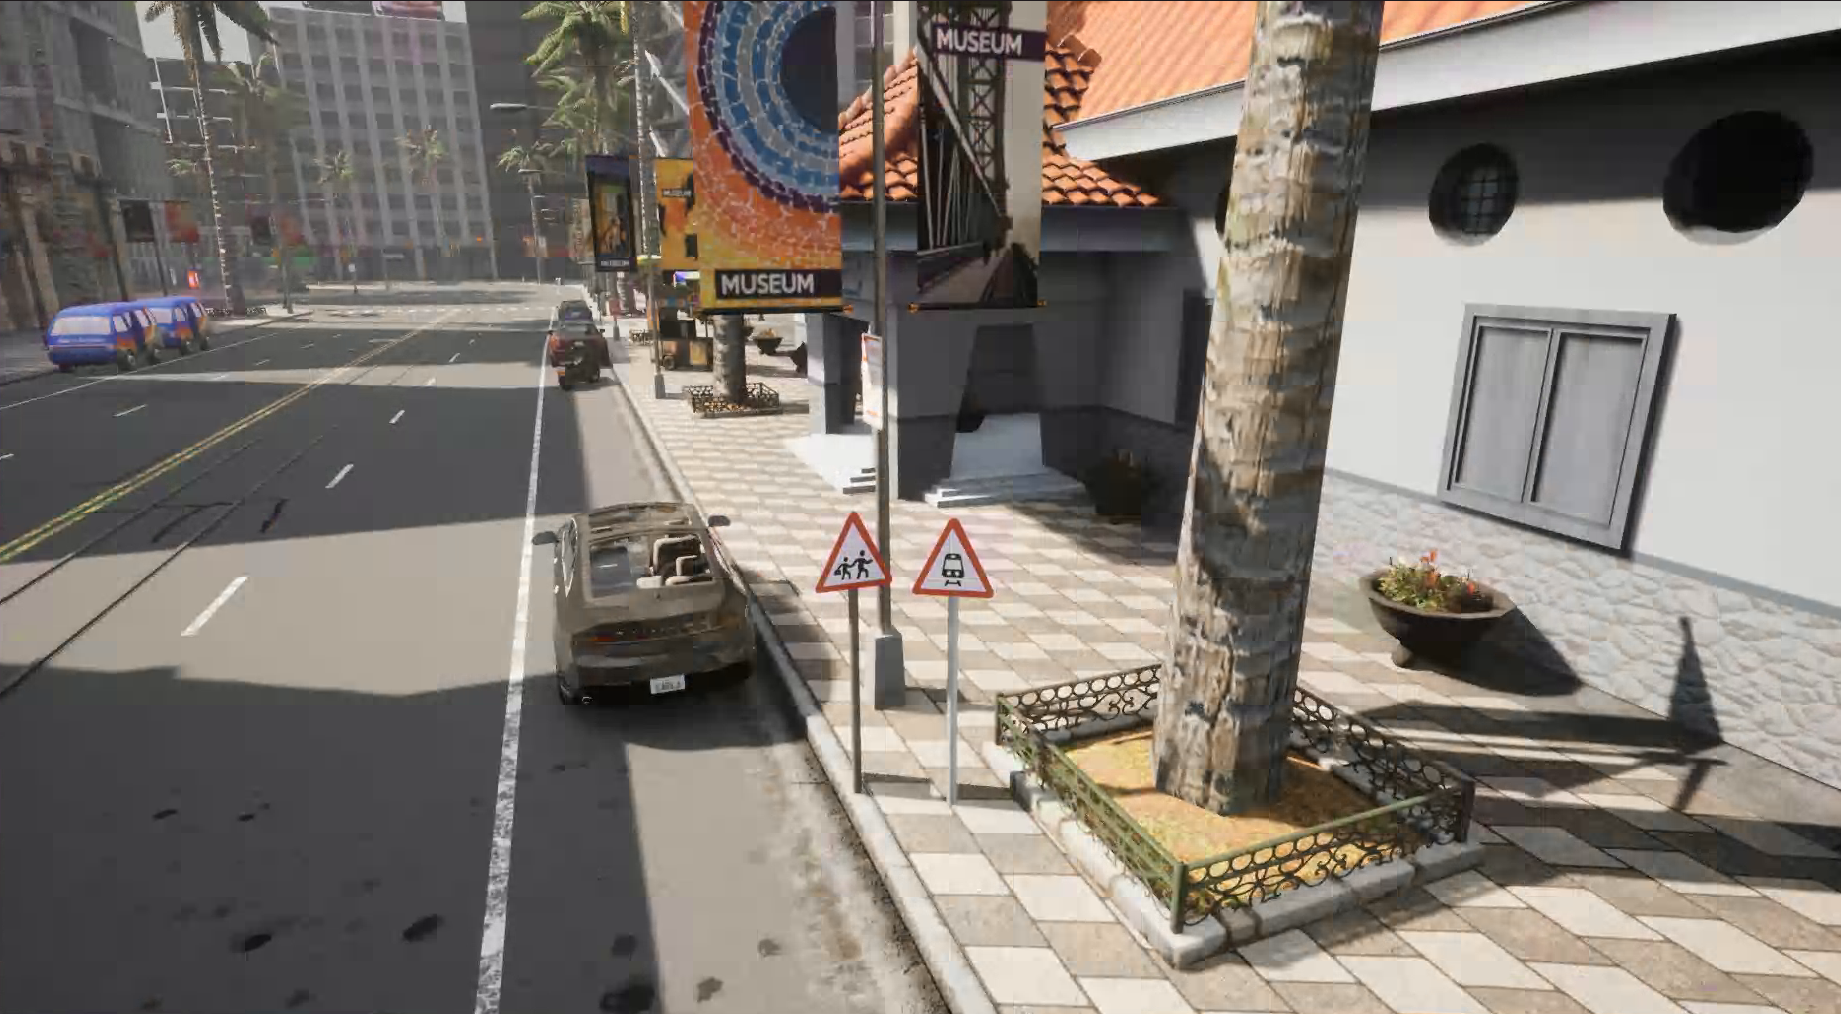
\includegraphics[width=0.45\textwidth]{resources/chapter-4/rambu-1.png}}
    \hfill
    \subfloat[]{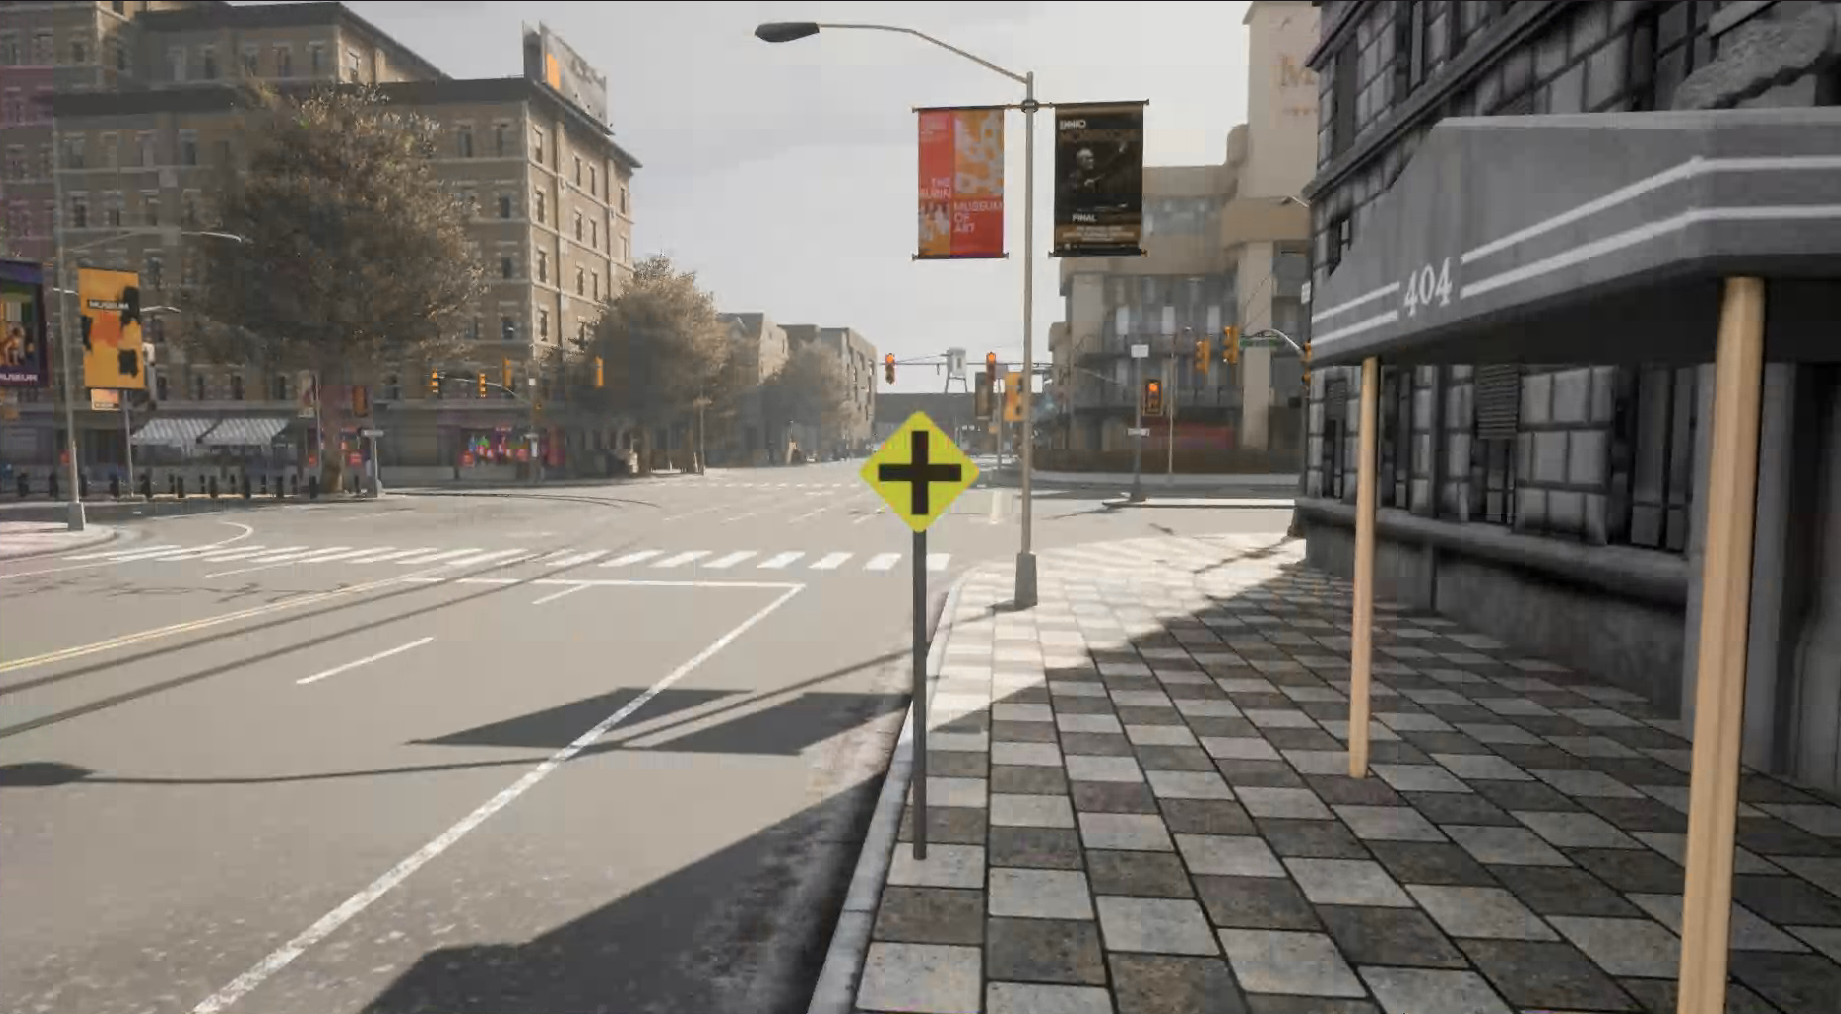
\includegraphics[width=0.45\textwidth]{resources/chapter-4/rambu-2.png}}
    \caption{Implementasi rambu-rambu lalu lintas dalam lingkungan simulasi}
    \label{fig:road-signs}
\end{figure}

\subsubsection{Rel}
% import mesh sebagai objek statis
% spline: butuh banyak edge/verts
% topview + stasiun

Gambar \ref{fig:rel} dan Gambar \ref{fig:rel-2} menunjukkan hasil implementasi rel.

% rel (lihat Gambar \ref{fig:rel-model}).

% \begin{figure}[!h]
%     \centering
%     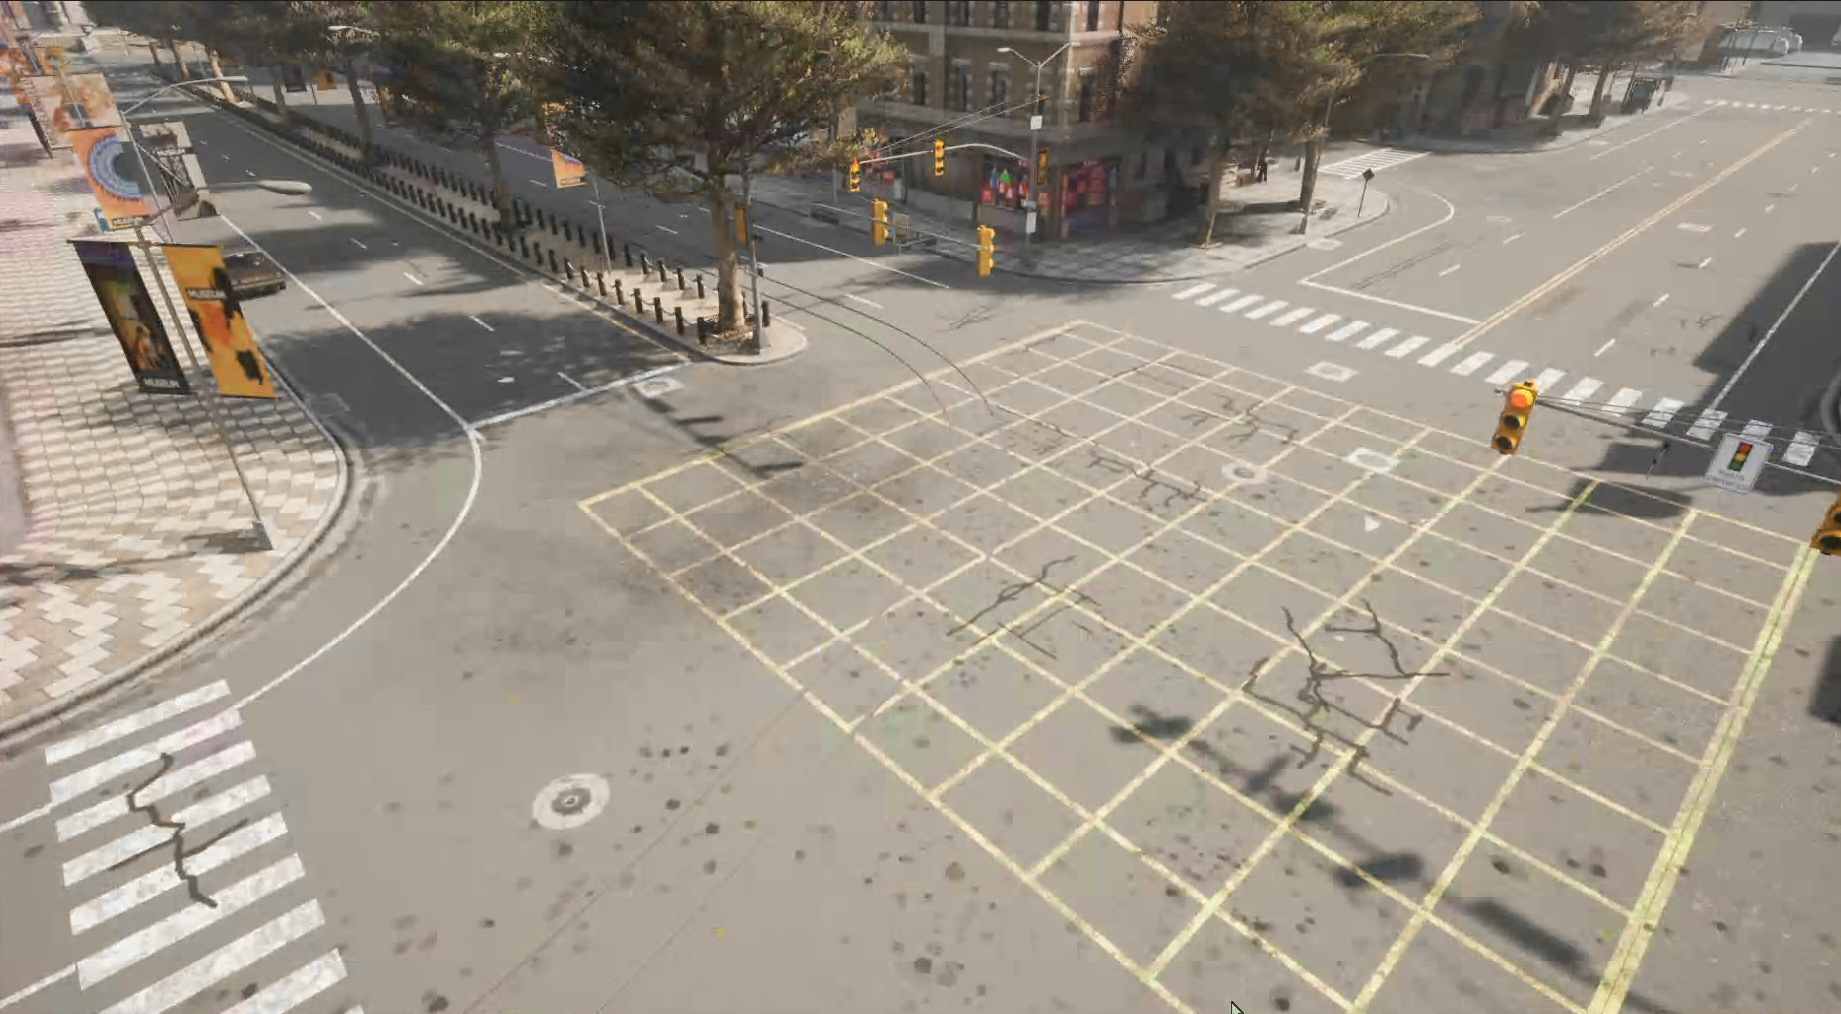
\includegraphics[width=0.6\textwidth]{resources/chapter-4/rel.png}
%     \caption{Implementasi rel dalam lingkungan simulasi}
%     \label{fig:rel-model}
% \end{figure}

\begin{figure}[!h]
    \centering
    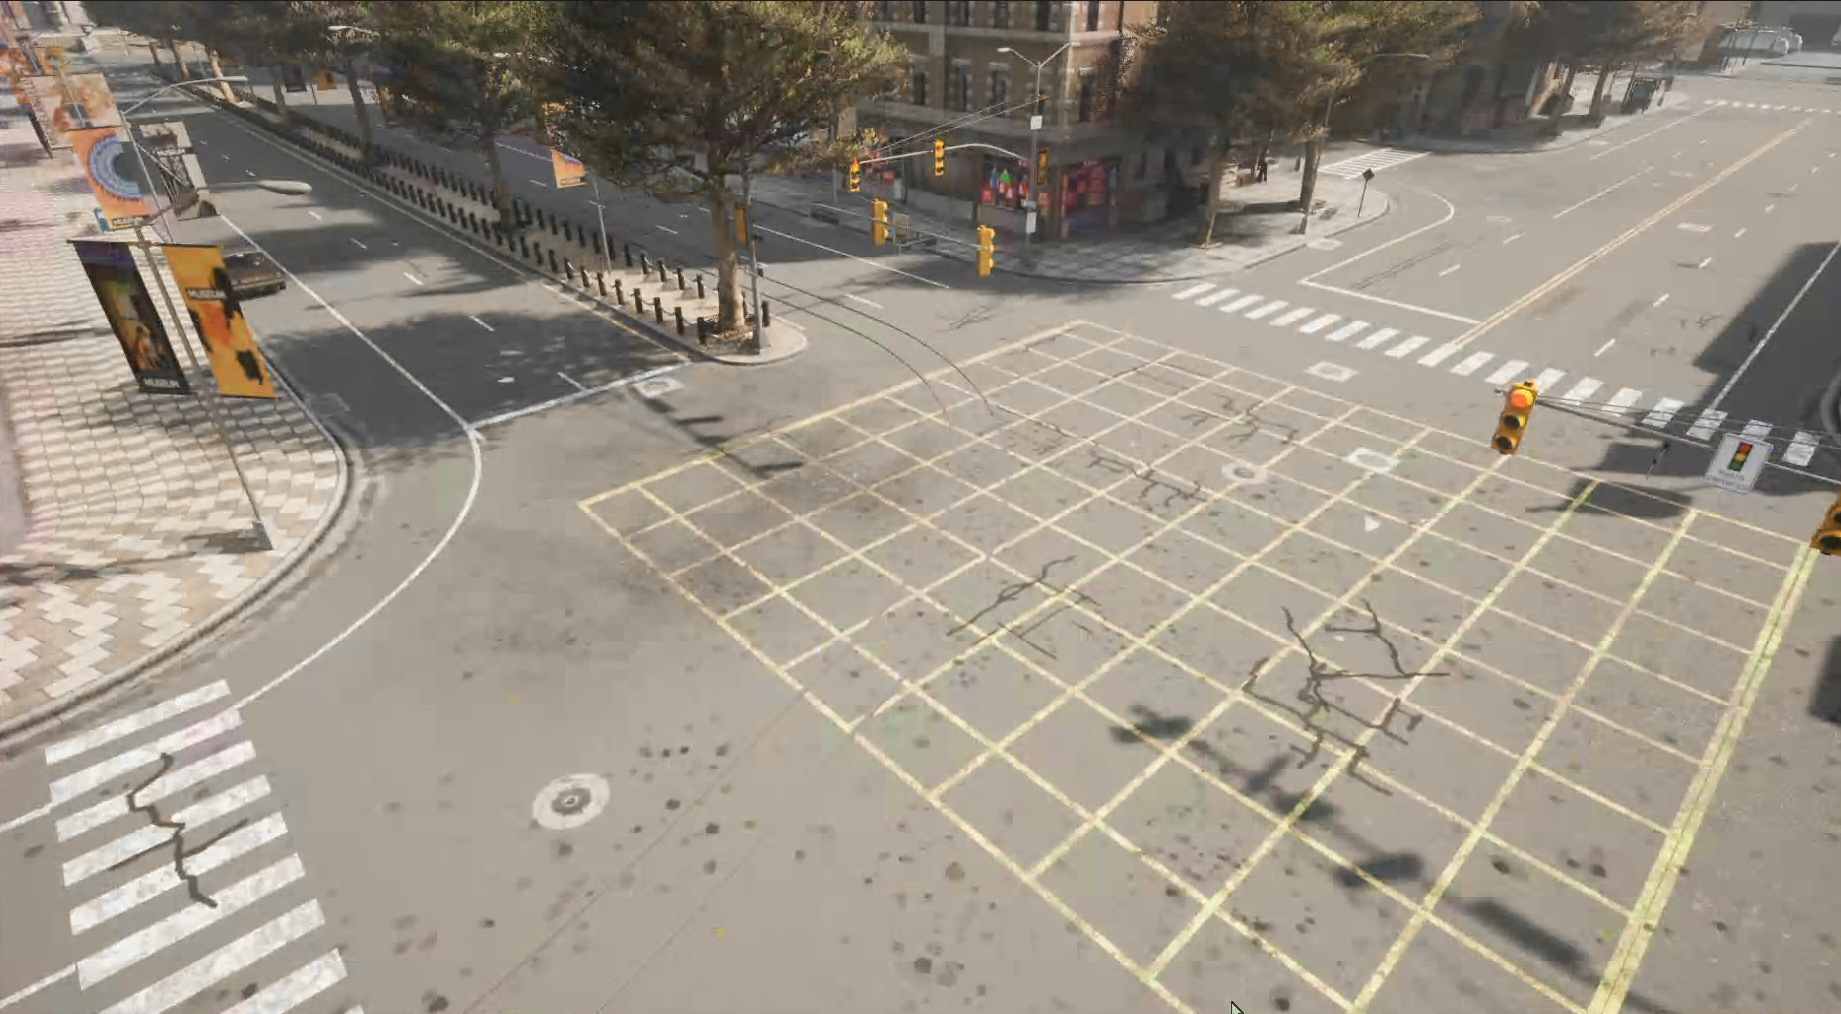
\includegraphics[width=0.6\textwidth]{resources/chapter-4/rel.png}
    \caption{Implementasi rel dalam lingkungan simulasi}
    \label{fig:rel}
\end{figure}

\begin{figure}[!h]
    \centering
    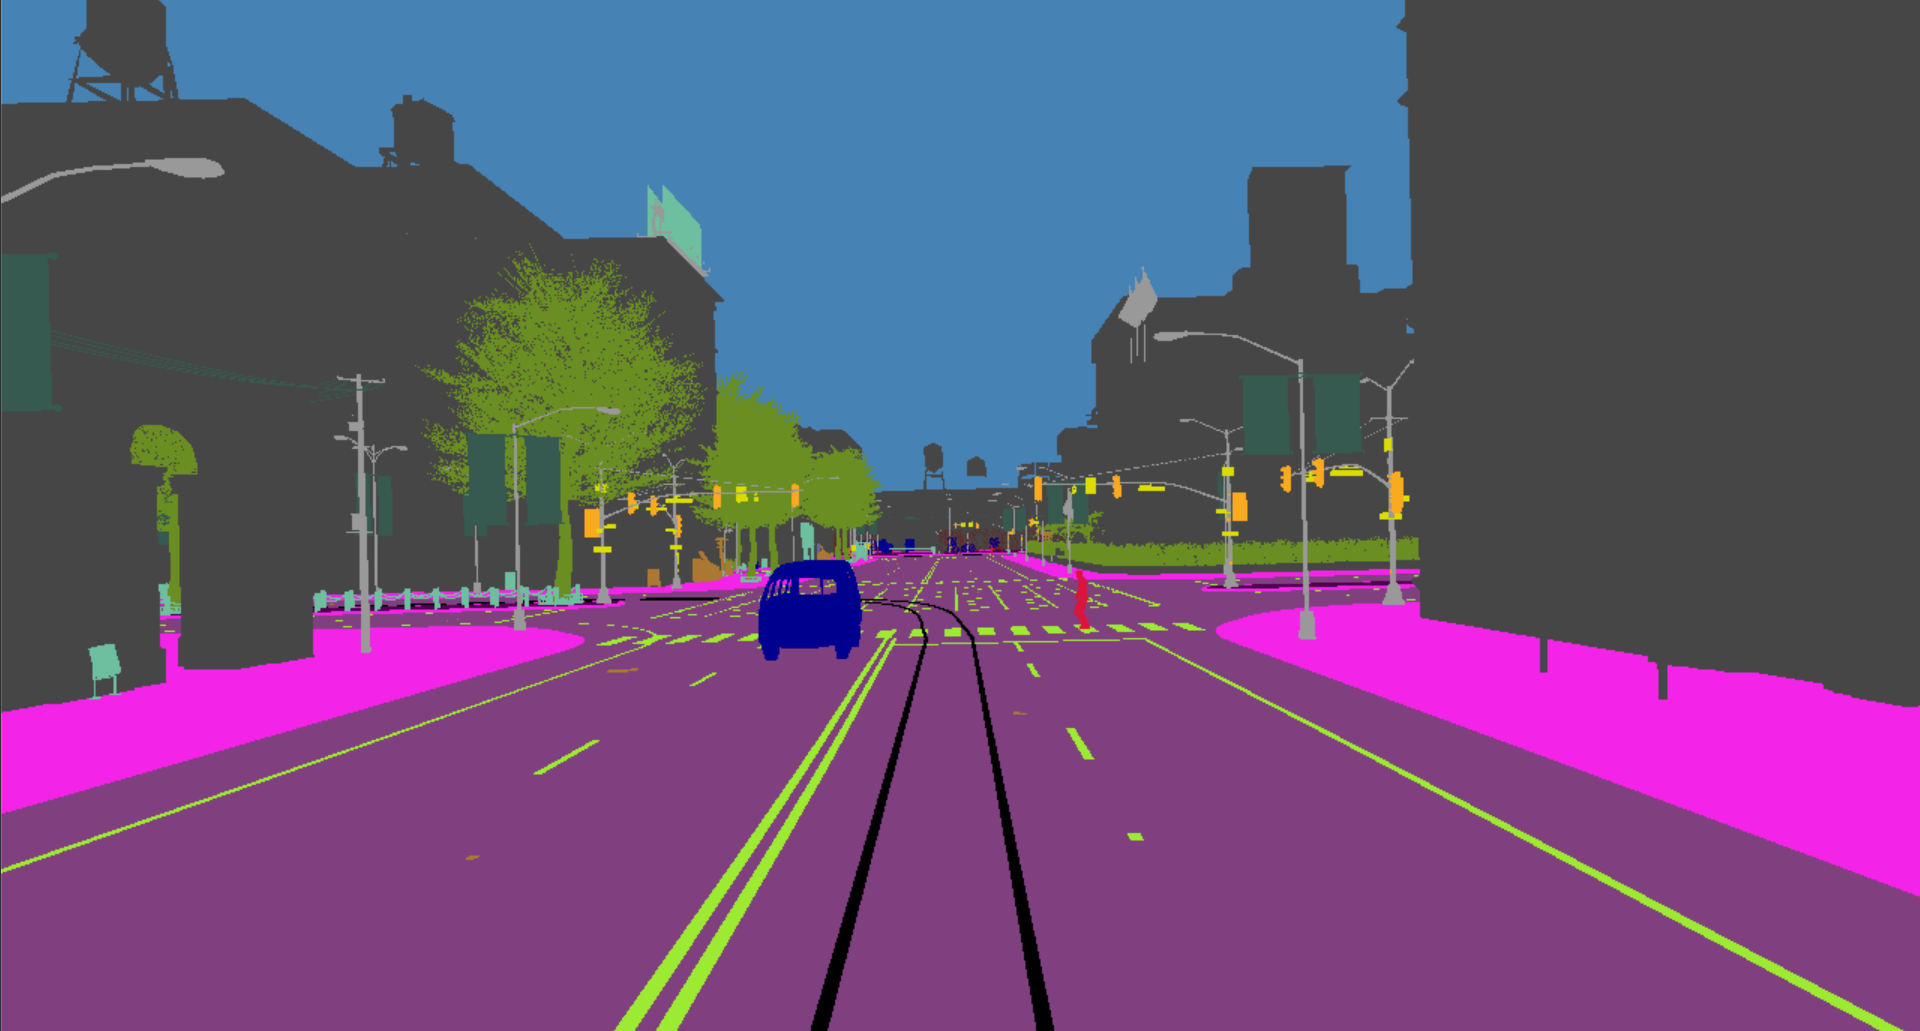
\includegraphics[width=0.6\textwidth]{resources/chapter-4/rel-segmentation-camera.png}
    \caption{Implementasi rel dalam lingkungan simulasi (tampilan segmentasi semantik)}
    \label{fig:rel-2}
\end{figure}

\section{Validasi}

\subsection{Tujuan Validasi}

Tujuan validasi adalah untuk memastikan bahwa objek-objek berperilaku normal
(seperti aslinya) dan stabil saat simulasi berjalan.

% TODO: lengkapin

\subsection{Hasil Validasi}
% manual + generate

\section{Distribusi Hasil Implementasi}

% TODO: hasil ss

\section{Evaluasi}
% kendaraan roda 2 dan 3 berhasil diimplementasikan namun tidak stabil
% ? tidak diperlukan perta
% tidak diperlukan data OpenDRIVE untuk traffic signs, karena:
% - tidak dibutuhkan
% - dari sisi trem, hanya butuh secara visual saja
% - dari sisi kendaraan lain (untuk autopilot), tidak dibutuhkan juga, mostly cuman penanda ada ini
